\documentclass[doktyp=barbeit]{TUBAFarbeiten}

\usepackage[ngerman,english]{babel}

\usepackage{selinput}% Auswahl der Dateikodierung (ansi,latin1,utf8,...)
	\SelectInputMappings{adieresis={ä},germandbls={ß},Euro={€}}% Zeichenzuordnung für selinput.sty
\usepackage[T1]{fontenc}% Einstellung Fontencoding

\usepackage{csquotes}% Einstellung zu Anführungszeichen; wird von biblatex.sty gefordert
\usepackage[backend=biber,style=numeric,sorting=none,sortlocale=de_DE_phonebook]{biblatex}% bessere Literaturverarbeitung
\addbibresource{literaturquellen.bib}

\usepackage{hyperref}
\usepackage[table,figure]{hypcap}

\usepackage{tabularx,diagbox}
\usepackage{float}

\usepackage{amsmath}

\usepackage{listings}
\definecolor{gray}{rgb}{0.95,0.95,0.95}
\definecolor{violet}{rgb}{0.5, 0.0, 0.6}
\lstset{ basicstyle=\ttfamily\small, backgroundcolor=\color{gray} }
\lstset{ numbers=left, numberstyle=\tiny, numbersep=2pt }
\lstset{ breaklines=true, keywordstyle=\color{violet} }

%\usepackage{setspace}% Einstellungen Zeilenabstand
	%\onehalfspacing% Einstellungen Zeilenabstand

\setcounter{secnumdepth}{4}
% \setcounter{tocdepth}{4}

% Worttrennung für nicht bekannte Wörter
\hyphenation{Con-nect-able}
\hyphenation{Es-tab-lish-ment}
\hyphenation{Mode}
\hyphenation{Ad-ver-tise-ment}



\TUBAFFakultaet{Fakultät für Mathematik und Informatik}
\TUBAFInstitut{Institut für Informatik}
\TUBAFLehrstuhl{Lehrstuhl für Betriebssysteme und Kommunikationstechnologien}

%\TUBAFZweitlogo{\includegraphics{thekla_logo.jpg}}

\TUBAFTitel[Entwicklung einer Sicherheitsinfrastruktur zur Bluetooth-Kommunikation zwischen Smartphone und Mikrocontroller]{Entwicklung einer Sicherheitsinfrastruktur zur Bluetooth-Kommunikation zwischen Smartphone und Mikrocontroller}
\TUBAFBetreuer{\,Prof.\,Dr. Konrad Froitzheim}
\TUBAFKorrektor{M.Sc. Jonas Treumer}%TODO Betreuer Lorenzo Neumann
\TUBAFAutor[M. Käsemodel]{Marian Käsemodel}
\TUBAFStudiengang{Angewandte Informatik}
\TUBAFVertiefung{Technik}
\TUBAFMatrikel{62\,412}
\TUBAFDatum[]{\today}%TODO

\begin{document}

\maketitle

\TUBAFErklaerungsseite


\KOMAoptions{
	listof=totoc	% Abbildungs- und Tabellenverzeichnis im Inhaltsverzeichnis
}

\tableofcontents
\newpage
\listoffigures
\listoftables

\newpage
\section{Einleitung}
	\label{sec: einleitung}
	\textit{Bluetooth} ist eine weit verbreitete Kommunikationstechnologie, die von vielen Geräten wie Smartphones, Laptops und eingebetteten Systemen unterstützt wird. Seit 2010 unterteilt sich \textit{Bluetooth} in die Varianten \textit{Bluetooth Classic} und \textit{Bluetooth Low Energy}. Zweiteres ist eine geeignete Alternative für Geräte, die einen niedrigen Energieverbrauch anstreben.
\\\\
Viele Infrastrukturen, die auf \textit{Bluetooth} basieren, transportieren sensible Daten. Bekannte Anwendungen sind Smartwatches, die mit Smartphones kommunizieren, oder die Vernetzung von eingebetteten Systemen in der Industrie. Ein weiterer Anwendungsfall sind autonome Verleihdienste für Kleinfahrzeuge innerhalb von Städten. So können Personen Fahrräder oder Roller ausleihen, um flexibel am Individualverkehr teilzunehmen. Einige dieser Dienste verwenden dabei \textit{Bluetooth}, um zwischen dem Fahrzeug und dem Smartphone des Nutzers Daten zu übertragen. Für diese Anwendungen, stellt sich die Frage, welche Sicherheiten \textit{Bluetooth} bietet.
\\\\
Hintergrund dieser Arbeit ist das Projekt \textit{SteigtUM}, das einen solchen autonomen Verleih umsetzen soll. Es unterscheidet sich von anderen Verleihdiensten durch die Nutzung von Lastenfahrrädern. Dabei soll ein neuer Anwendungsfall berücksichtigt werden, der es dem Nutzer ermöglicht, das Fahrrad abzustellen und zu einem späteren Zeitpunkt wiederzuverwenden. Auf diese Weise kann der Nutzer bspw. zu einem Geschäft gelangen, Einkäufe tätigen und diese anschließend nach Hause transportieren. Im Rahmen dieser Arbeit wird die Idee verfolgt, dass das Smartphone des Nutzers mit dem Mikrocontroller des Fahrzeugs über \textit{Bluetooth Low Energy} kommuniziert.

	\subsection{Problemstellung}
		\label{sec: problemstellung}
		Ziel der Arbeit ist zunächst die Untersuchung der Schwachstellen innerhalb von \textit{Bluetooth Low Energy}. Dazu muss ein tieferes Verständnis für dessen Funktionsweise und die zur Verfügung gestellten Sicherheitsfunktionen gewonnen werden. Auf diesem Wissen aufbauend wird eine Infrastruktur entworfen, durch die ein Smartphone und ein Mikrocontroller mittels \textit{Bluetooth Low Energy} sicher miteinander kommunizieren können. Weder bei der Übertragung noch bei der Verarbeitung innerhalb des Systems soll eine außenstehende Instanz auf die übertragenen Nachrichten zugreifen können. Demnach ist eine Lösung für die Probleme der Authentizität, Datenintegrität und Vertraulichkeit erforderlich. Im Idealfall ist die Infrastruktur nicht nur auf die Geräte Smartphone und Mikrocontroller beschränkt, sondern wäre für jede Art von Bluetooth-Gerät denkbar.
\\\\
Desweiteren ist es Ziel der Arbeit, mithilfe dieser Infrastruktur eine Implementierung umzusetzen, die sich auf das Projekt \textit{SteigtUM} bezieht. Da bei dem vorgestellten Verleihdienst sensible Daten zwischen Smartphone und Fahrzeug ausgetauscht werden, wird die Infrastruktur als Grundlage für die sichere Kommunikation genutzt. Dennoch sind weitere Lösungen gefordert. Nur der Nutzer darf Zugriff auf die Funktionen des ausgeliehenen Fahrzeugs erlangen. Demnach muss zu Beginn eines Ausleihprozesses sichergestellt werden, dass der Nutzer berechtigt ist, das Fahrzeug auszuleihen. Verlässt er das Fahrzeug und möchte es nach einer bestimmten Zeit wieder nutzen, soll kein anderer in der Lage sein, das Fahrzeug in der Zwischenzeit zu entsperren und zu entwenden.

\newpage
\section{Grundlagen zu Bluetooth Low Energy}
\label{sec: grundlagen le}

	\subsection{Überblick}
		\label{sec: le ueberblick}
		Bluetooth ist ein Industriestandard für die Übertragung von Daten per Funk, dessen Intention die Reduzierung von Kabelverbindungen an mobilen sowie stationären Geräten ist. Wichtige Eigenschaften der Technologie sind vor allem ein niedriger Energieverbrauch und günstig herstellbare Hardware. Seit 1998 wird Bluetooth von der \textit{Bluetooth Special Interest Group} (SIG) entwickelt und ist seit 2002 von der \textit{Organisation Institute of Electrical and Electronics Engineers} (IEEE) standardisiert \cite{IEEE}.
% QUELLE https://standards.ieee.org/standard/802_15_1-2002.html)
\\\\
Es agiert im lizenzfreien ISM-Band (Industrial, Scientific and Medical Band) von 2,4 GHz. 
% TODOOPT QUELLE
% BR/EDR: BT Specification 4.0 PDF S. 124, 1.1 Overview of BR/EDR Operation, 1. Absatz
% LE: BT Specifiaction 4.0 PDF S. 126, 1.2 OVERVIEW OF BLUETOOTH LOW ENERGY OPERATION, 1. Absatz
Zur Reichweite kann keine genaue Aussage getroffen werden, da sie von vielen Parametern wie beispielsweise der Sendeleistung und Einflüssen aus der Umwelt abhängt. Um trotzdem einen Eindruck zu gewinnen, kann für bestimmte Bedingungen und Konfigurationen die maximale Reichweite mithilfe eines Tools \cite{BtRangeTool} der SIG ermittelt werden. Dabei variieren die Ergebnisse von ca. einem Meter bis hin zu mehr als 1000 Metern.
% QUELLE https://www.bluetooth.com/learn-about-bluetooth/key-attributes/range/
\\\\
Grundlegend wird Bluetooth seit der Version 4.0 von 2010 in die zwei Systeme \textit{Basic Rate} (BR) und \textit{Low Energy} (LE) unterteilt, wobei LE darauf ausgelegt ist, weniger Energie als BR zu benötigen. Die neueste Bluetooth"=Version ist die Version 5.2, die wie jede Version abwärtskompatibel ist. Jedoch sind beide Systeme (BR und LE) bezüglich der Kommunikation miteinander inkompatibel: implementiert ein Gerät nur das BR"=System, kann es keine Daten mit einem Gerät austauschen, das nur das LE"=System unterstützt. Demnach ist für LE die Abwärtskompatibilität nur bis zur Version 4.0 gegeben. Desweiteren ist es möglich, dass ein Gerät über beide Systeme verfügt und so die meisten Nutzungsfälle abdeckt. Das BR"=System kann mit den Erweiterungen \textit{Enhanced Data Rate} (EDR) und \textit{Alternate Media Access Control and Physical Layer} (AMP) genutzt werden, um eine höhere Datenrate zu erzielen. Die einzelnen Systeme und Erweiterungen können entsprechend ihrer Bluetooth-Version die in Tabelle \ref{tab: maximale Bitraten BT} dargestellten Datenraten erreichen.
\begin{table}[H]
    \begin{tabular}[h]{|l|l|l|}
    \hline
    \textbf{System/Erweiterung} & \textbf{max. Bitrate (Version 4.0)} & \textbf{max. Bitrate (Version 5.2)} \\
    \hline
    BR          & 1 Mbit/s \cite{BtSpec4.0_124}               & 1 Mbit/s \cite{BtSpec5.2_188}           \\
    \hline
    BR/EDR      & 2 Mbit/s bis 3 Mb/s \cite{BtSpec4.0_124}    & 2 Mbit/s bis 3Mb/s \cite{BtSpec5.2_188} \\
    \hline
    802.11 AMP  & 24 Mbit/s \cite{BtSpec4.0_123}              & 52 Mbit/s \cite{BtSpec5.2_187}          \\
    \hline
    LE          & 1 Mbit/s \cite{BtSpec4.0_126}               & 2 Mbit/s \cite{BtSpec5.2_190}           \\
    \hline
    % QUELLE
    % BT Specification 4.0 PDF S. 124, 1.1 Overview of BR/EDR Operation, 1. Absatz
    %                          S. 126, 1.2 OVERVIEW OF BLUETOOTH LOW ENERGY OPERATION, 1. Absatz
    % BT Specification 5.2 PDF S. 188 1.1 Overview of BR/EDR Operation, 1. Absatz
    %                          S. 190, 1.2 OVERVIEW OF BLUETOOTH LOW ENERGY OPERATION, 1. Absatz
    \end{tabular}
    \caption[Maximale Bitraten der Bluetooth-Systeme]{Maximale Bitraten der Bluetooth-Systeme}
    \label{tab: maximale Bitraten BT}
\end{table}
\textit{Da Bluetooth Low Energy (BLE) ein zentraler Bestandteil dieser Arbeit ist, bezieht sich der Autor von nun an nur darauf und nicht mehr auf Bluetooth im Allgemeinen. D.h., dass Bluetooth Classic, welches BR/EDR und AMP beschreibt, nur noch behandelt wird, wenn das BR"=System oder eine seiner Erweiterungen explizit erwähnt werden.}
\\\\
Die Architektur eines Bluetooth"=Systems unterteilt sich in einen Host und in einen oder mehrere Controller. Ein Host ist eine logische Entität, definiert als alle Schichten unterhalb der nicht zu Bluetooth gehörigen Profile (Protokolle) und oberhalb des Host"=Controller"=Interface (HCI). Ein Controller ist eine logische Entität, definiert als alle Schichten bzw. Funktionsblöcke unterhalb des HCI. Der Aufbau setzt sich immer aus genau einem primären Controller und optional aus sekundären Controllern zusammen. Dabei kann die Rolle des primären Controllers entweder durch einen BR/EDR"=Controller, einen LE"=Controller oder durch eine Kombination aus BR/EDR- und LE"=Controller eingenommen werden, während die Rolle eines sekundären Controllers nur durch einen AMP"=Controller besetzt werden kann. In Abb. \ref{fig: kombinationen aus host und controller} sind einige Varianten skizziert. 
% TODOOPT QUELLE BT Specification 4.0, PDF S.123 f.
\begin{figure}[H]
    \centering
    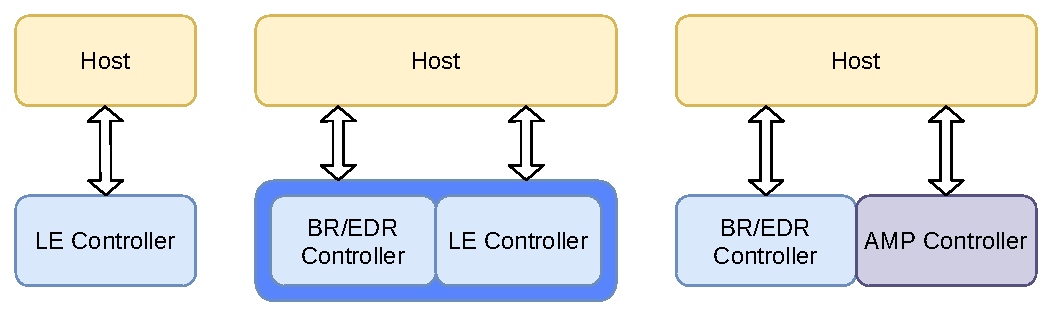
\includegraphics[width=0.9\linewidth]{graphics/kombination_host_controller.pdf}
    \caption[Kombinationen aus Host und Controller]{Kombinationen aus Host und Controller; in Anlehnung an \cite{BtSpec4.0_fig_124}}
    \label{fig: kombinationen aus host und controller}
\end{figure}
% QUELLE BILD BT Sepcification 4.0, PDF S. 124
Zur Veranschaulichung der Architektur bezüglich eines LE"=Systems ist in der Abb. \ref{fig: host controller architektur} die Zusammensetzung aus Host und Controller mit deren Schichten bzw. Protokollen festgehalten, die in den Sektionen \ref{sec: le controller} und \ref{sec: le host} thematisiert werden. Über dem Host befindet sich die Anwendungsschicht.
\begin{figure}[H]
    \centering
    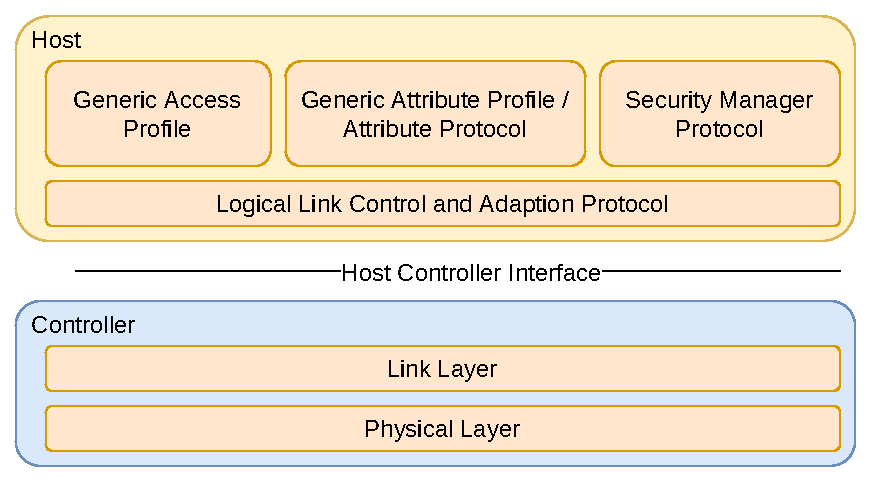
\includegraphics[width=0.7\textwidth]{graphics/host_controller_hci.pdf}
    \caption[BLE-Architektur von Host und Controller]{BLE-Architektur von Host und Controller; in Anlehnung an \cite{BtSpec4.0_fig_137}}
    \label{fig: host controller architektur}
\end{figure}

	\subsection{Topologie}
		\label{sec: le topologie}
		Die Topologie der Infrastruktur beschränkt sich auf das Minimum an Kommunikationsparteien und ist unabhängig von der Anwendung.\\

% TODO BILD topologie infratruktur mikrocontroller, smartphone, CA

Dem Thema zufolge sollen ein Mikrocontroller und ein Smartphone sicher Daten austauschen. Um dies zu bewerkstelligen, wird über den Transport der Daten durch Bluetooth Low Energy (BLE) das Verschlüsselungsprotokoll TLS verwendet (siehe Sektion X). 
% TODO SEKTION VERWEIS Infrakstruktur->Sicherheit
Dementsprechend ist, wie in Abbildung X zu sehen
% TODO BILD VERWEIS topologie infrastruktur mikrocontroller, smartphone, CA
, neben dem Mikrocontroller und dem Smartphone eine Zertifizierungsstelle notwendig. In welcher Form diese auftritt ist von der Anwendung abhängig.

Für einen seriösen Anwendungsfall sollte die Zertifizierungsstelle evtl. in Form eines Servers existieren, der dem Mikrocontroller und Smartphone in regelmäßigen Abständen (z.B. jährlich) jeweils ein Zertifikat ausstellt. Mit diesen Zertifikaten und der Kenntnis über das Root-Zertifikat können Mikrocontroller und Smartphone sich gegenseitig authentifizieren und somit die Grundlage für eine sichere Kommunikation bilden.

Beispielsweise könnte es für einen privaten Anwendungsfall ausreichend sein, die Zertifizierungsstelle nicht als dauerhaft betriebenen Server darzustellen, sondern lediglich ein Root-Zertifikat zu erstellen und mit diesem dem Mikrocontroller und Smartphone jeweils ein digitales Zertifikat auszustellen.

Die Rolle der Partei, die die Zertifikate für Mikrocontroller und Smartphone austellt muss nicht zwingend eine Zertifizierungsstelle sein, sondern könnte auch eine Entität sein, der von einer Zertifizierungsstelle ein Zwischenzertifikat ausgestellt wurde.

	\subsection{Verbindungsaufbau}
		\label{sec: le verbindungsaufbau}
		Um mittels BLE ein Piconet zu bilden, ist ein Advertiser notwendig. Auf drei vorgegebenen Frequenzen, den Advertising Channels (siehe Sektion \ref{sec: le phy channel}), sendet er Daten, mit denen er sich für andere Geräte bemerkbar macht (Advertisements). Dabei können Advertisements auch genutzt werden, um Nutzdaten zu senden. Jedes Advertisement-Paket beinhaltet eine Bluetooth-Adresse des Senders, die 48 Bit lang ist.
\\\\
Geräte, die Daten auf den Advertising Channels empfangen, werden Scanner bzw. Initiator genannt. Auf diesem Weg finden sich die Geräte (Discovering). Der Initiator unterscheidet sich vom Scanner, da er in der Lage ist, sich zu einem Advertiser zu verbinden, von dem er ein Advertisement erhalten hat, das eine Verbindung ermöglicht. Sind zwei Geräte verbunden, senden und empfangen sie ihre Pakete auf den Data Channels (siehe Sektion \ref{sec: le phy channel}). Verbinden sich zwei Geräte, wird der Initiator als Master und der Advertiser als Slave angesehen.
\\\\
Durch die Anwendung von Zeitmultiplexing senden die Geräte ihre Pakete immer zu festgelegten Zeitpunkten. Dabei ist ein Event ein zeitlicher Abschnitt, in dem zusammenhängende Daten in Form von Paketen gesendet bzw. empfangen werden.

\begin{figure}[H]
    \centering
    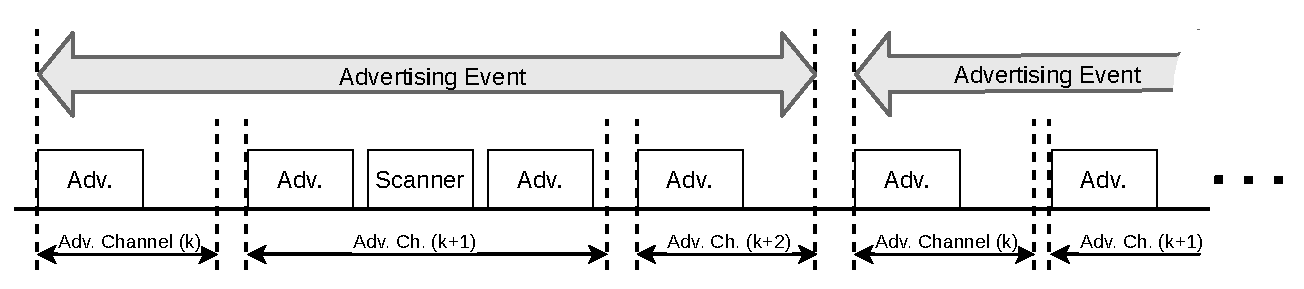
\includegraphics[width=\textwidth]{graphics/advertising_event.pdf}
    \caption[Advertising Event]{Advertising Event \cite{BtSpec4.0_127}}
    \label{fig: adv event}
\end{figure}
% QUELLE Spec S. 127 oben

In Abb. \ref{fig: adv event} ist ein Advertising Event dargestellt, bei dem ein Advertiser auf allen drei Advertising Channels nacheinander Advertisement-Pakete sendet. Auf dem zweiten Kanal empfängt der Advertiser -direkt im Anschluss auf sein erstes Advertisement-Paket- in diesem Kanal ein Paket eines Scanners, auf das er mit einem weiteren Advertisement antwortet.

\begin{figure}[H]
    \centering
    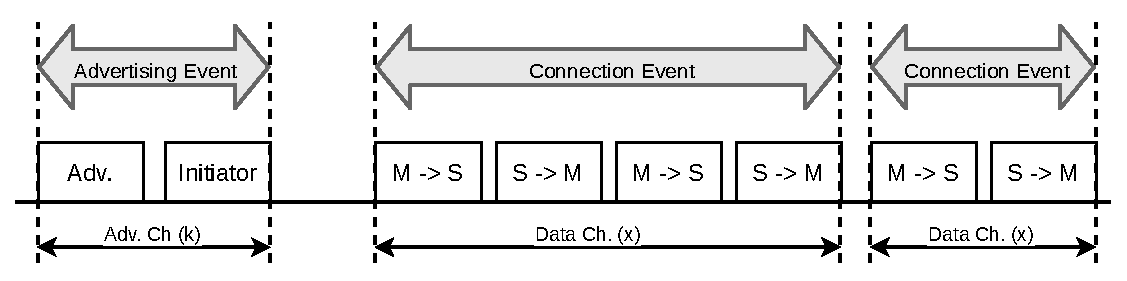
\includegraphics[width=0.9\textwidth]{graphics/advertising_initiator_event.pdf}
    \caption[Advertising und Connection Event]{Advertising und Connection Event \cite{BtSpec4.0_127}}
    \label{fig: adv init}
\end{figure}
% QUELLE Spec S. 127 unteres bild

In Abbildung \ref{fig: adv init} ist ein Advertising Event dargestellt, bei dem ein Initiator auf das Advertisement-Paket eines Advertiser antwortet, um eine Verbindung aufzubauen. Darauf folgt ein Connection Event, bei dem Master (ursprünglich Initiator) und Slave (ursprünglich Advertiser) einander Pakete auf einem Data Channel senden. Danach folgt ein weiteres Connection Event auf einem anderen Data Channel.

	\subsection{Controller}
		\label{sec: le controller}
		Wie in Abbildung X
% TODO BILD VERWEIS letztes Bild aus überblick
zu sehen ist, umfasst der Controller die Schichten Physical Layer (PHY) und Link Layer (LL, auch Logical Layer genannt). Der Phyical Layer unterteilt sich weiter in die Physical Channels und die Phyical Links, während der Link Layer sich in Logical Transports und Logical Links aufteilt. In den Schichten bzw. ihren Untergliederungen wird definiert, wie Anwenderdaten, Advertisements und Kontrollsignale in Form von Unicasts bzw. Broadcasts übertragen werden.

% TODO ABBILDUNG physical layer, physical channel/transports, link layer, locigal transports/links
% TODO evtl zum Bild anmerken, dass L2CAP nicht zum Controller sondern zum Host gehört

		\subsubsection{Physical Layer}
			\label{sec: le phy}

			\paragraph{Physical Channel} \mbox{} \vspace{0.2cm} \\
				\label{sec: le phy channel}
				Um miteinander zu kommunizieren, müssen zwei Bluetooth"=Geräte (ein Sender und ein Empfänger) zur selben Zeit den selben Kanal nutzen, wobei sich der Empfänger in der Reichweite des Senders befinden muss. Da mehrere Piconets zur selben Zeit im selben lokalen Bereich agieren können, besteht die Wahrscheinlichkeit, dass zwei Sender zweier verschiedener Gerätepaare in Reichweite den selben Kanal zur selben Zeit nutzen und eine Kollision verursachen.
\\\\
Mittles des Frequenzmultiplexverfahrens ist das ISM"=Band eines LE"=Systems von 2400 MHz bis 2483,5 MHz in 40 Funkkanäle unterteilt. Beginnend bei 2402 MHz nutzt jeder Kanal eine Frequenz, die 2 MHz über der Frequenz des Vorgängers liegt. Das Trägersignal wird mithilfe des Gaussian Frequency Shift Keying moduliert. \cite{BtSpec4.0_2180-2181}
% QUELLE Specification 4.0 PDF S. 2180-2181

Somit bildet der Physical Channel die niedrigste Ebene der Architektur. 37 der 40 Kanäle werden als LE Piconet Channel (entsprechend S. \pageref{fig: controller architektur} Abb. \ref{fig: controller architektur} als LE Piconet Physical Channel) bezeichnet, die mit einem Piconet assoziiert werden und zur Kommunikation zwischen zwei bereits verbundenen Geräten dienen. Die verbleibenden drei Kanäle werden Advertisement Broadcast Channel (entsprechend S. \pageref{fig: controller architektur} Abb. \ref{fig: controller architektur} als LE Advertising Physical Channel) genannt und befinden sich auf den Frequenzen 2402 MHz, 2426 MHz sowie 2480 MHz. \cite{BtSpec4.0_2199}
% QUELLE advertisment frequenzen Specification 4.0 PDF S. 2199
\\\\
Mittels Advertisements können Geräte in diesen drei Kanälen auf sich aufmerksam machen, um von anderen Geräten entdeckt zu werden. Zudem werden sie genutzt, um Geräte miteinander zu verbinden oder Anwendungsdaten an Scanner bzw. Initiatoren zu senden. Ein Gerät kann nur einen Kanal zur selben Zeit nutzen, weswegen das Zeitmultiplexverfahren verwendet wird, das bereits verbundenen Geräten ermöglicht, zusätzlich das Advertisement zu betreiben.
\\\\
Um Interferenzen innerhalb des genutzten Frequenzbands z.B. mit \textit{Wi-Fi} zu vermeiden, wird das Adaptive Frequency Hopping \cite{BtAfh} genutzt (eine Form des Frequency Hopping Spread Spectrum). Dabei wechseln Sender und Empfänger in kurzen Zeitabständen den Kanal und passen die Menge der zu nutzenden Kanäle (Channel Map) an, indem sie dynmaisch ermittleln, in welchen Kanälen häufiger Kollisionen auftreten. Treten in einem Kanal häufig Interferenzen auf, wird er für eine bestimmte Zeitspanne aus der Channel Map entfernt und vorerst nicht mehr genutzt.
% QUELLE https://www.bluetooth.com/blog/how-bluetooth-technology-uses-adaptive-frequency-hopping-to-overcome-packet-interference/

			\paragraph{Physical Link} \mbox{} \vspace{0.2cm} \\
				\label{sec: le phy link}
				Ein Physical Link wird immer mit genau einem Physical Channel assoziiert. Dagegen kann ein Physical Channel mehrere Physical Links unterstützen. Bezüglich Bluetooth wird der Physical Link nicht in der Struktur eines Paketes repräsentiert, kann aber innerhalb eines LE-Paketes anhand der Access Address identifiziert werden. \cite{BtSpec4.0_164}
\\\\
Active Physical Links sind die Punkt-zu-Punkt-Verbindungen zwischen Master und Slave über einen Piconet Physical Channel und gelten nur als aktiv, wenn ein Asynchronous Connection (ACL) Logical Transport zwischen den Geräten existiert. \cite{BtSpec4.0_166-167}

Advertising Physical Links dienen dazu, zwischen einem Advertiser und einem Initiator einen Active Physical Link aufzubauen, und existieren nur für einen kurzen Zeitraum. Zwischen Advertiser und Scanner existieren sie für längere Zeit und dienen dem Broadcast von Nutzdaten. \cite{BtSpec4.0_166-167}

		\subsubsection{Link Layer}
			\label{sec: le ll}

			\paragraph{Paketstruktur}
				\label{sec: le ll paketstruktur}
				Der Link Layer nutzt ein gemeinsames Paketformat für das Übertragen von Advertising"=Paketen und Nutzdaten"=Pakten, das in Abb. \ref{fig: ll paket struktur} dargestellt ist.\\
\begin{figure}[H]
    \centering
    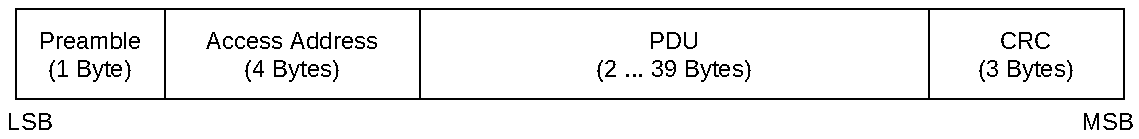
\includegraphics[width=0.9\textwidth]{graphics/link_layer_packetformat.pdf}
    \caption[Paketstruktur des Link Layers]{Paketstruktur des Link Layers; in Anlehnung an \cite{BtSpec4.0_fig_2200}}
    \label{fig: ll paket struktur}
\end{figure}
% QUELLE Spec 4.0 S. 2200 - 2201
Die Preamble hat eine Größe von acht Bit und wird genutzt, um auf Empfängerseite die Frequenz zu synchronisieren, die Zeiteinteilung der Symbole zu schätzen und um die Automatic Gain Control zu trainieren. Die Preamble beträgt immer 0b01010101, falls das Bit mit dem niedrigsten Stellenwert (LSB für Least Significant Bit) der Access Address 1 ist. Anderenfalls beträgt die Preamble 0b10101010. \cite{BtSpec4.0_2200-2201}
\\\\
Die Access Address hat eine Größe von 32 Bit und identifziert eine Verbindung über den Link Layer bzw. dient dazu, Pakete mittels des festgelegten Wertes 0x8E89BED6 als Advertisement"=Pakete zu identifzieren. Bevor ein Initiator eine Verbindung zu einem Advertiser aufbaut, erstellt er eine zufällige Access Address, die neben weiteren Bedingungen nicht der des Advertisement"=Pakets gleichen oder sich nur um ein Bit von ihr unterscheiden darf. Diese Access Address sendet er dann innerhalb der Verbindungsanfrage an den Advertiser. \cite{BtSpec4.0_2200-2201}
\\\\
Das letzte Feld des Link"=Layer"=Pakets ist der 24 Bit lange Cyclic Redundancy Check (CRC), der über das PDU"=Feld berechnet wird. Im Fall, dass auf Ebene des Link Layers die PDU verschlüsselt wird, generiert man den CRC erst nach der Verschlüsselung. Unabhängig davon, ob die Verschlüsselung aktiv ist, wird anschließend ein Whitening \cite{BtSpec4.0_2217-2218} durchgeführt, um Sequenzen vieler gleichbleibender Bit (bspw. 0b00000000) zu verhindern. \cite{BtSpec4.0_2200-2201}
% QUELLE Spec 4.0 S. 2217-2218
\\\\
Die Protocol Data Unit (PDU) unterteilt sich in die Advertising Channel PDU und Data Channel PDU.

\subparagraph{Advertising Channel PDU} \mbox{} \vspace{0.2cm} \\
Wie in Abb. \ref{fig: ll adv channel pdu} gezeigt wird, besteht die Advertising Channel PDU aus einem 16 Bit langen Header und einem Payload variabler Länge. RFU steht dabei für Reserved for Future Use.
\begin{figure}[H]
    \centering
    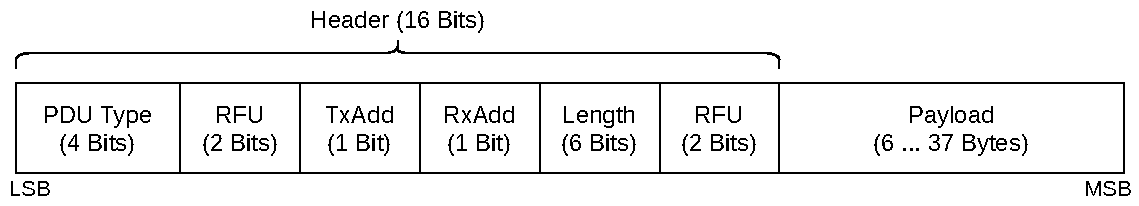
\includegraphics[width=0.9\textwidth]{graphics/link_layer_packetformat_pdu_adv.pdf}
    \caption[Link Layer Advertising Channel PDU]{Link Layer Advertising Channel PDU; in Anlehnung an \cite{BtSpec_fig_2201} und \cite{BtSpec_fig_2202}}
    \label{fig: ll adv channel pdu}
\end{figure}
% QUELLE advertising channel pdu format S. 2201 f.
Dabei beinhaltet der Header unter anderem ein 4 Bit langes Feld für den PDU Type (bspw. Connectable Undirected Advertising Event oder Scan Request) und zwei Flags TxAdd und RxAdd für zusätzliche Informationen bezüglich des PDU Type. Die Bedeutungen von TxAdd und RxAdd hängen vom PDU Type ab. Die Menge aller PDU Types lässt sich folgendermaßen untergliedern:
\begin{itemize}
    \item Advertising PDU
    \item Scanning PDU
    \item Initiating PDU
\end{itemize}
Bei allen bilden die ersten 6 Byte des Payload die Adresse des Senders (Advertiser, Scanner oder Initiator). Hier sagt TxAdd bei jedem PDU Type aus, ob die angegebene Adresse des Senders öffentlich (TxAdd = 0) oder zufällig generiert (TxAdd = 1) ist. Diese Funktion wird Privacy Feature gennant und ist in Sektion \ref{sec: gap sicherheit} genauer beschrieben. RxAdd dagegen ist nur bei PDU Types von Bedeutung, die in ihrem Payload eine zweite Adresse enthalten, nämlich die des Empfängers. Analog zu TxAdd sagt RxAdd aus, ob die Adresse des Empfängers öffentlich (RxAdd = 0) oder zufällig (RxAdd = 1) ist.
\\\\
Ein weiteres Feld im Header der Advertising Channel PDU ist das 6 Bit lange Feld für die Länge des Payloads in Byte, dessen Wert eine Spanne von 6 bis 37 Byte abdeckt. \cite{BtSpec4.0_2201-2208}
\\\\
\subparagraph{Data Channel PDU} \mbox{} \vspace{0.2cm} \\
Die Data Channel PDU nutzt entsprechend der Abb. \ref{fig: ll data channel pdu} einen 16 Bit langen Header, einen Payload variabler Länge und optional einen 32 Bit langen Message Integry Check (MIC), der die Integrität des Payload sicherstellt. Das MIC"=Feld entfällt bei einer unverschlüsselten Link"=Layer"=Verbindung und bei einer Data Channel PDU, deren Payload leer ist.
\begin{figure}[H]
    \centering
    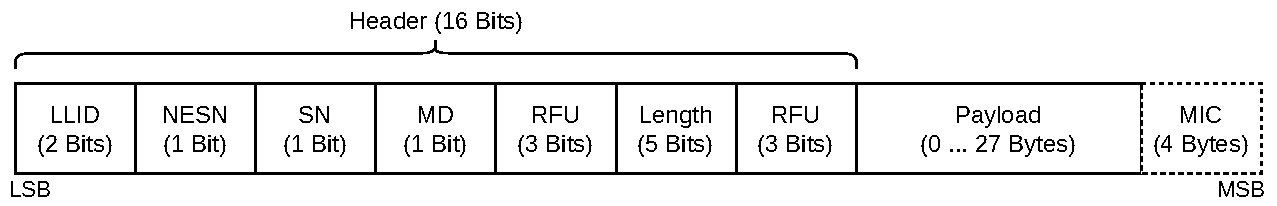
\includegraphics[width=1\textwidth]{graphics/link_layer_packetformat_pdu_data.pdf}
    \caption[Link Layer Data Channel PDU]{Link Layer Data Channel PDU; in Anlehnung an \cite{BtSpec_fig_2208a} und \cite{BtSpec_fig_2208b}}
    \label{fig: ll data channel pdu}
\end{figure}
Das erste Feld des Headers ist der zwei Bit lange Link Layer Identifier (LLID), der mit 0b01 sowie 0b10 aussagt, dass es sich um eine LL Data PDU handelt und mit 0b11, dass es sich um eine LL Control PDU handelt. Der Wert 0b00 ist reserviert. Die LL Control PDU dient dazu, die LL"=Verbindung zu steuern. Dazu gehören unter anderem Anfragen zum Ändern der Verbindungsparameter (z.B. Window Size oder Timeout), zum Ändern der Channel Map oder zum Verschlüsseln.
\\\\
Auf die LLID folgt das Feld der Next Expected Sequence Number (NESN) und das Feld der Sequence Number (SN) mit jeweils einem Bit Länge, die innerhalb Sektion \ref{sec: le ll transport} näher erläutert werden.
\\\\
Unter anderem beinhaltet der Header ein fünf Bit langes Feld für die Länge des Payload in Byte und ggf. einschließlich der Länge des MIC. Der maximale Wert der Länge beträgt 31 Byte, wobei sich der Payload in jedem Fall auf eine maximale Länge von 27 Byte bemisst. \cite{BtSpec4.0_2208-2209}
\\\\
In der Bluetooth-Version 4.2 ist das Feld der Länge auf acht Bit erweitert, wodurch der Payload eine maximale Größe von 251 Byte annehmen kann. \cite{BtSpec4.2_2589-2590}

			\paragraph{Logical Transport} \mbox{} \vspace{0.2cm} \\
				\label{sec: le ll transport}
				Über dem Physical Layer baut sich der Link Layer auf, beginnend mit dem Logical Transport, der sich in die zwei Arten LE Asynchronous Connection (LE ACL) und LE Advertising Broadcast (ADVB) unterteilt.

Die LE ACL transportiert Kontrollsignale des über ihr befindlichen Logical Link und Logical Link Control and Adaption Protocol (L2CAP). Außerdem überträgt die LE ACL asynchrone Anwenderdaten nach dem Best-Effort-Prinzip.

Mithilfe der Next Expected Sequence Number bzw. Sequence Number (NESN/SN), die jeweils nur die Größe eines Bits besitzen, wird eine einfache Zuverlässigkeit gewährleistet. Empfängt ein Gerät ein Paket B, vergleicht es dessen NESN mit der SN, die es innerhalb des vorherigen Pakets A abgesendet hat. Wenn diese unterschiedlich sind, wurde das vorherige Paket A vom Gegenüber vollständig und korrekt empfangen (ACK für Acknowledgement). Anderenfalls sind die Nummern gleich, was bedeutet, dass das vorherige Paket A nicht vollständig bzw. korrekt empfangen wurde (NACK/NAK für Negative Acknowledgement) und nun erneut an den Gegenüber gesendet werden muss. Zudem prüft das Gerät die SN des empfangenen Pakets B mit der NESN seines vorher gesendeten Pakets A. Sind diese Nummern gleich, wurde das empfangene Paket B vom Gerät erwartet. Anderenfalls sind die Nummern verschieden und somit wurde das Paket B nicht erwartet, weswegen es ignoriert wird. Somit wird auch die Flusskontrolle ermöglicht, da ein Empfänger bei nicht ausreichend freiem Speicher im Buffer ein NACK mithilfe der Sequenznummern zurücksenden kann.
% TODO QUELLE evtl mit BILD: NESN/SN 4.0 PDF S. 2240 f.

Wenn ein Gerät einem Piconet beitritt, wird zwischem dem Master und dem Slave eine Default LE ACL über einen Active Physical Link gebildet. Die Default LE ACL ist einer Access Address zugeordnet. Wird die Default LE ACL getrennt, werden alle Logical Transports zwischen Master und Slave getrennt. Bei einem unerwarteten Synchronisationsverlust zum LE Piconet Physical Channel werden der LE Physical Link und alle LE Logical Transports und LE Logical Links entfernt.

Der ADVB transportiert ohne Verwendung von Acknowledgements Kontrollsignale und Anwenderdaten bezüglich des Broadcasts über den darunter gelegenen LE Advertising Broadcast Link. Der Datenverkehr ist überwiegend unidirektional, ausgehend vom Advertiser zu allen in Reichweite befindlichen Scannern. Scanner können eine Anfrage an den Advertiser senden, um weitere Anwenderdaten über den Broadcast zu empfangen oder um eine LE ACL zu bilden. Aufgrund des Verzichts auf Acknowledgements ist der ADVB unzuverlässig, weswegen Pakete redundant übertragen werden. Sobald ein Gerät mit dem Advertising beginnt, wird ein ADVB erzeugt, der anhand der Adresse des Gerätes identifiziert wird.
% TODO QUELLE allg. für paragraph: Specification 4.0 PDF S. 174

			\paragraph{Logical Link} \mbox{} \vspace{0.2cm} \\
				\label{sec: le ll link}
				Ein Logical Link unterscheidet sich je nachdem, ob er auf einem LE ACL Logical Transport oder einem ADVB Logical Transport aufbaut und ob er zur Übertragung von Kontrollsignalen oder Nutzdaten genutzt wird. Anhand des Logical Link Identifier (LLID) im Header des Basisbandpakets (siehe S. \pageref{fig: ll data channel pdu} Abb. \ref{fig: ll data channel pdu}) wird unterschieden, ob es sich bei der zu übertragenden PDU um Nutzdaten oder Kontrollsignale handelt.

Der Control Logical Link (LE-C) nutzt den darunter liegenden LE ACL Logical Transport, um Kontrollsignale zwischen Geräten im Piconet zu übertragen.

Der User Asynchronous Logical Link (LE-U) nutzt den darunter liegenden LE ACL Logical Transport, um alle asynchronen Nutzdaten zu übertragen. Über dem Link Layer agiert das Protokoll L2CAP, dessen Frame für den Link Layer fragmentiert werden müssen. Mithilfe des LLID-Wertes 0b10 wird der Beginn eines L2CAP-Frame (das erste Fragment eines L2CAP-Frame) und der Wert 0b01 die Fortsetzung eines L2CAP-Frame (die folgenden Fragmente des L2CAP-Frame) gekennzeichnet. Somit wird der Header des Protokolls L2CAP einfach gehalten und eine korrekte Synchronisation bei der Zusammensetzung der Fragmente zu einem L2CAP-Frame garantiert. Jedoch muss folglich ein L2CAP-Frame vollständig übertragen werden, bevor ein neues übertragen wird.

Der Advertising Broadcast Control Logical Link (ADVB-C) nutzt den darunter liegenden Default ADVB, um Kontrollsignale für Verbindungsanfragen oder Anfragen für weitere Broadcast-Nutzdaten zu übertragen.

Der Advertising Broadcast User Data Logical Link (ADVB-U) nutzt den darunter liegenden Default ADVB, um verbindungslos und ohne den Gebrauch von LE-U Nutzdaten als Broadcast zu senden. \cite{BtSpec4.0_176-177}
% QUELLE paragraph: Specification 4.0, S.176 f.

	\subsection{Host}
		\label{sec: le host}
		Im Wesentlichen umfasst der Host das Logical Link Control and Adaption Protocol (L2CAP), das Generic Access Profile (GAP) und Generic Attribute Profile (GATT) sowie das Security Manager Protocol (SMP). Er liegt unter der Anwendungsebene und steuert den Datentransport als auch den Verbindungsaufbau sowie Sicherheitsaspekte. Je nachdem wie Host und Controller implementiert sind, kann das standarisierte Host Controller Interface (HCI) als Schnittstelle zwischen Host und Controller dienen. Es ist optional \cite{BtSpec4.0_138}, da es Implementierungen bestehend aus Host und Controller gibt, die direkt verbunden sind, so dass ein HCI nicht nötig ist. Da das HCI den allgemeinen Kommunikationsprozess zwischen Bluetooth-Geräten nicht nennenswert beeinflusst, wird es hier nicht weiter behandelt.

		\subsubsection{Logical Link Control and Adaption Protocol}
			\label{sec: le l2cap}
			Das Logical Link Control and Adaption Protocol (L2CAP) bildet die unterste Schicht im Host (siehe S. \pageref{fig: host controller architektur} Abb. \ref{fig: host controller architektur}) und dient je nach Konfiguration dazu, den Datenverkehr zu steuern und zwischen höheren und niedrigeren Schichten zu vermitteln. Mittels Multiplexing können mehrere Anwendungen einen LE-U (also Logical Link) nutzen.
% TODOOPT QUELLE Spec 4.0 S. 1400 2.3 Operation Between Layers
Es verfügt über fünf Modi:
\begin{itemize}
    \item Basic L2CAP Mode
    \item Flow Control Mode
    \item Retransmission Mode
    \item Enhanced Retransmission Mode
    \item Streaming Mode
    \item LE Credit Based Flow Control Mode (seit Bluetooth 4.2)
\end{itemize}
Für Bluetooth allgemein (BR/EDR und LE) wird immer der Basic L2CAP Mode genutzt, wenn kein anderer festgelegt wird. Der LE Credit Based Flow Control Mode soll \cite{BtSpec4.2_1735} zufolge als einziger Modus für verbindungsorientierte LE"=Kanäle genutzt werden ("`This is the only mode that shall be used for LE L2CAP connection oriented channels"' \cite{BtSpec4.2_1735}). Da diese Aussage nicht ausschließt, dass eine verbindungsorientierte LE"=Verbindung über den standardmäßig festgelegten Basic L2CAP Mode erfolgen kann, und der LE Credit Based Flow Control Mode noch nicht in der Bluetooth"=Version 4.0 vertreten war \cite{BtSpec4.0_1401}, ist anzunehmen, dass eine verbindungsorientierte LE"=Verbindung auch mit dem Basic L2CAP Mode möglich ist.
% QUELLE ZITAT Spec. 4.2 S. 1735
% QUELLE Spec 4.0 S. 1401
\\\\
Logische Kanäle, genannt L2CAP Channels, dienen innerhalb eines Geräts als Endpunkt für höher gelegene Protokolle oder direkt für die Anwendung und sind für jedes Gerät individuell an dem Channel Identifier (CID) unterscheidbar. Folglich muss der L2CAP Channel einer Verbindung zwischen zwei Geräten von diesen nicht zwingend mit der gleichen CID gekennzeichnet sein.
% TODOOPT QUELLE Spec. 4.0 S. 1390
\\\\
Der L2CAP Layer wird von zwei Modulen gesteuert: dem Resource Manager und dem Channel Manager (siehe Abb. \ref{fig: l2cap architektur}).

\begin{figure}[H]
    \centering
    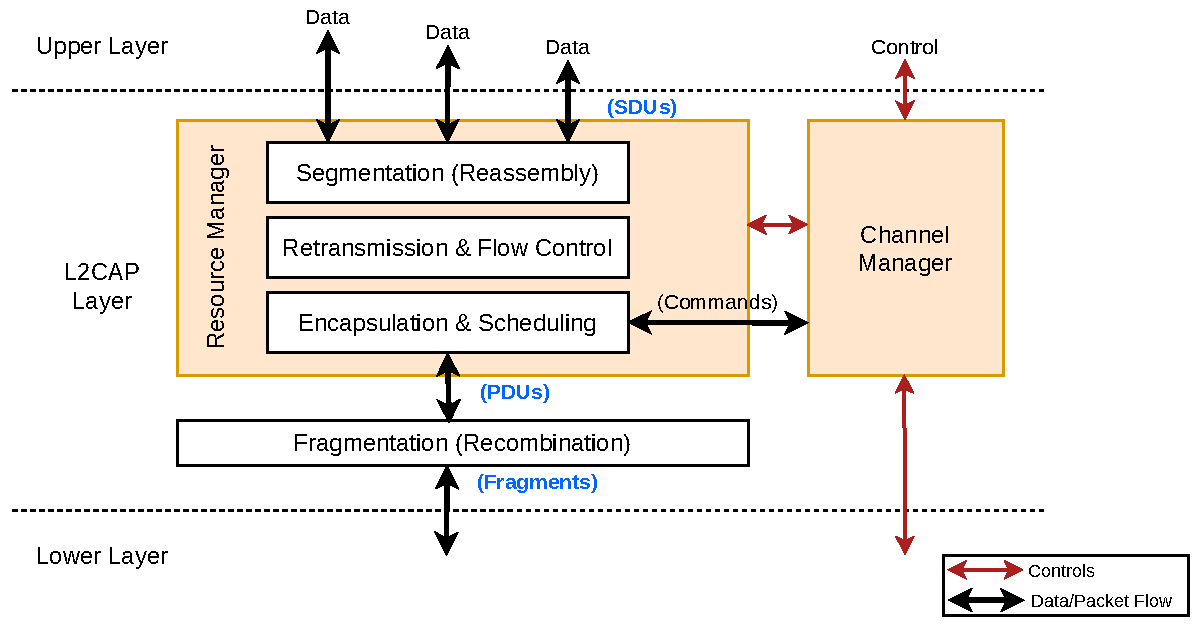
\includegraphics[width=0.9\textwidth]{graphics/l2cap_architektur.pdf}
    \caption[Architektur des L2CAP Layers]{Architektur des L2CAP Layers \cite{BtSpec4.0_1391}}
    \label{fig: l2cap architektur}
\end{figure}
% QUELLE l2cap layer resource manager channel manager spec 4.0 S. 1391

Der Channel Manager ist für die Verwaltung und Steuerung der L2CAP Channels zuständig. Das umfasst die auf L2CAP bezogene Signalübertragung intern, Peer"=to"=Peer, und zu höheren und niedrigeren Schichten \cite{BtSpec4.0_1390}. 
% QUELLE Spec. 4.0 S. 1390
Die Signale, die zwischen den zwei L2CAP"=Entitäten zweier verbundenen Geräte übertragen werden, sind Kommandos wie bspw. der LE Credit Based Connection Request und die entsprechende Response. Dafür wird ein separater L2CAP Channel mit der CID 0x0005 genutzt. Zudem betreibt der Channel Manager den L2CAP"=Zustandsautomaten, auf den hier nicht näher eingegangen werden soll.
\\\\
Da der L2CAP Layer nach unten mit dem Link Layer verknüpft ist (ggf. über das HCI), müssen die L2CAP PDUs dem Paketformat des Link Layers (bzw. dem HCI) gerecht werden. Dementsprechend werden die L2CAP PDUs fragmentiert bzw. wieder zusammengesetzt. Die Maximal PDU Payload Size (MPS) bezeichnet die maximale Größe des Payload einer PDU in Byte, die eine L2CAP"=Entität verarbeiten kann.
% TODOOPT BILD + VERWEIS Spec 4.0 S. 1487, Mischung aus Figure 7.1 und 7.2, vereinfacht darstellen: L2CAP PDU -> HCI Paket -> Link Layer Paket
\\\\
Ein Datenaustausch zwischen L2CAP und dessen höhergelegenen Schichten / Protokollen erfolgt in der Form von Service Data Units (SDU), wobei deren Ursprung immer aus einer höheren Schicht stammt. Die Maximum Transmission Unit (MTU) bezeichnet die maximale Größe einer SDU in Byte, die die höhergelegene Schicht verarbeiten kann. Die Segmentierung (bzw. Zusammensetzung) dieser SDUs wird vom Resource Manager ausgeführt und ist für alle Modi außer dem Basic L2CAP Mode relevant. Wenn keine Segementierung angewandt wird, ist die MTU gleich der MPS \cite{BtSpec4.2_1727}. Falls ein L2CAP Channel in einem anderen Modus als dem Basic L2CAP Modus agiert, ist der Resource Manager auch für die erneute Übertragung von PDUs und Flusskontrolle zuständig. Außerdem plant der Resource Manager zu welchem Zeitpunkt L2CAP Channel PDUs versenden können, um den L2CAP Channels mit Quality"=of"=Service"=Optionen genügend Ressourcen bezüglich der Buffer des Controllers freizugeben. \cite{BtSpec4.2_185} \cite{BtSpec4.2_1725-1726}

\paragraph{Struktur eines Datenpakets} \mbox{} \vspace{0.2cm} \\
Es existieren verschiedene Arten von L2CAP"=Datenpaketen, die den gennanten Modi zugeordnet sind. Der Basic L2CAP Mode unterstützt verbindungsorientierte und verbindungslose L2CAP Channel, während die restlichen Modi nur verbindungsorientierte L2CAP Channels nutzen.
In Abb. \ref{fig: l2cap pdu basic} ist die Paketstruktur einer L2CAP PDU im Basic L2CAP Mode (verbindungsorientiert) dargestellt.

\begin{figure}[H]
    \centering
    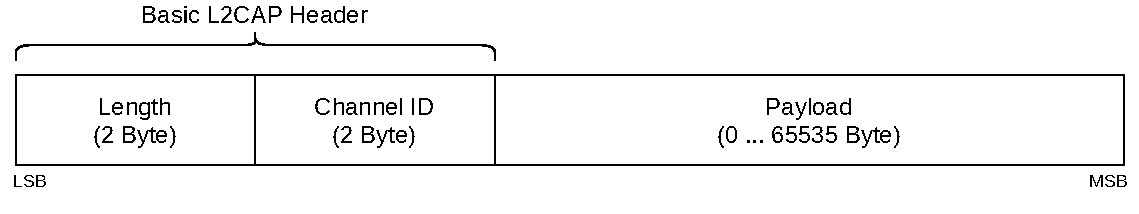
\includegraphics[width=0.9\textwidth]{graphics/l2cap_datenpaket.pdf}
    \caption[Struktur einer L2CAP PDU (Basic L2CAP Mode)]{Struktur einer L2CAP PDU (Basic L2CAP Mode) \cite{BtSpec4.2_fig_1737}}
    \label{fig: l2cap pdu basic}
\end{figure}
% QUELLE Spec. 4.2 S. 1737 Figure 3.1

LSB steht für Least Significant Bit, also das Bit mit niedrigstem Stellenwert, und MSB für Most Significant Bit, also das Bit mit höchstem Stellenwert. Das Längenfeld beschreibt die Länge des Payload, der eine maximale Länge von 65535 Byte besitzt.
\\\\
Abb. \ref{fig: l2cap pdu credit} zeigt die Paketstruktur einer L2CAP PDU im LE Credit Based Flow Control Mode.

\begin{figure}
    \centering
    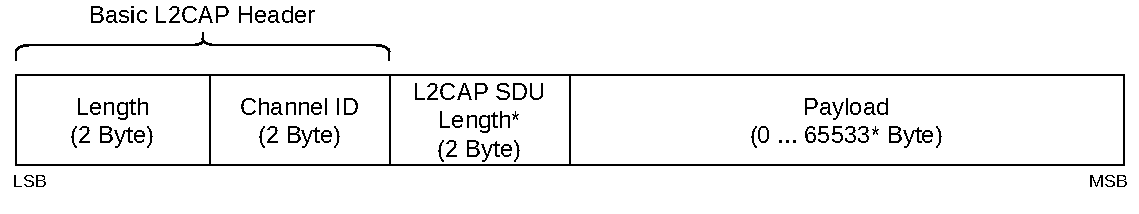
\includegraphics[width=0.9\textwidth]{graphics/l2cap_datenpaket_credit_based.pdf}
    \caption[Struktur einer L2CAP PDU (LE Credit Base Flow Control Mode)]{Struktur einer L2CAP PDU (LE Credit Base Flow Control Mode); *nur in erster PDU einer SDU; \cite{BtSpec4.2_fig_1747}}
    \label{fig: l2cap pdu credit}
\end{figure}
% QUELLE Spec 4.2 S. 1747 Figure 3.6

Das SDU"=Längenfeld ist nur in der ersten PDU einer SDU enthalten, um die Gesamtlänge der SDU in Byte zu beschreiben. Dadurch kann die Länge des Payloads einer solchen ersten PDU nur maximal 65533 Byte betragen, da der Wert des Längenfelds des Basic L2CAP Header auch das SDU"=Längenfeld umfasst. Alle zur SDU zugehörigen folgenden PDUs enthalten das SDU"=Längenfeld nicht, wodurch deren maximale Payload"=Länge 65535 Byte beträgt.

Im LE Credit Based Flow Control Mode regulieren die beiden Endpunkte mithilfe von Credits wie viele PDUs der jeweilige Endpunkt empfangen kann. Sind keine Credits mehr für einen Endpunkt (Empfänger) vorhanden, kann der andere Endpunkt (Sender) keine PDUs mehr an den Empfänger übermitteln und muss warten bis der Empfänger ein Credit"=Signalpaket sendet, das neue Credits freigibt. \cite{BtSpec4.2_1780}

		\subsubsection{Generic Attribute Profile}
			\label{sec: le gatt}
			Das Generic Attribute Profile (GATT) dient zur Kommunikation zwischen Client und Server. Es basiert auf dem Attribute Protocol (ATT), welches ausgehend vom Server Attribute bereitstellt, die von einem oder mehreren Clients "`entdeckt"' werden können. Ein Attribut besteht aus einem Typ, der anhand des Universal Unique Identifier (UUID) identifiziert wird, einem Attribute Handle, um auf das Attribut zuzugreifen, und einem Wert, der von Server und Client ausgelesen bzw. überschrieben werden kann. Zudem ist es möglich, für Attribute Berechtigungen festzulegen (bspw. nur Lesen, nicht Schreiben). \cite{BtSpec4.0_1835}
% QUELLE Spec 4.0 S. 1835 3.1 Introduction
\\\\
Entsprechend der S. \pageref{fig: host controller architektur} Abb. \ref{fig: host controller architektur} ordnet sich ATT über L2CAP in den Protokollstapel ein.
\\\\
Möchte ein Client einen Attributwert lesen bzw. schreiben, dann sendet er einen Read Request bzw. einen Write Request an den Server. Dieser reagiert, indem er bei einem Read Request das Attribut an den Client sendet bzw. bei einem Write Request den Attributwert entsprechend ändert und dem Client eine Bestätigung sendet. Im Fall, dass ausgehend vom Server ein Attribut geändert werden soll, sendet dieser eine Notification oder eine Indication an den Client. Im Gegensatz zur Notification bestätigt der Client eine empfangene Indication. \cite{BtSpec4.0_1854-1855} \cite{BtSpec4.0_1861-1863}
% QUELLE Spec 4.0 S. 1854 f. 3.4.4.3 Read Request und 3.4.4.4 Read Response
% QUELLE Spec 4.0 S. 1861-1863 3.4.5.1 Write Request und 3.4.5.2 Write Response
\\\\
Die Daten werden in Form von Attribute Protocol PDUs (siehe Abb. \ref{fig: att pdu}) übertragen.

\begin{figure}[H]
    \centering
    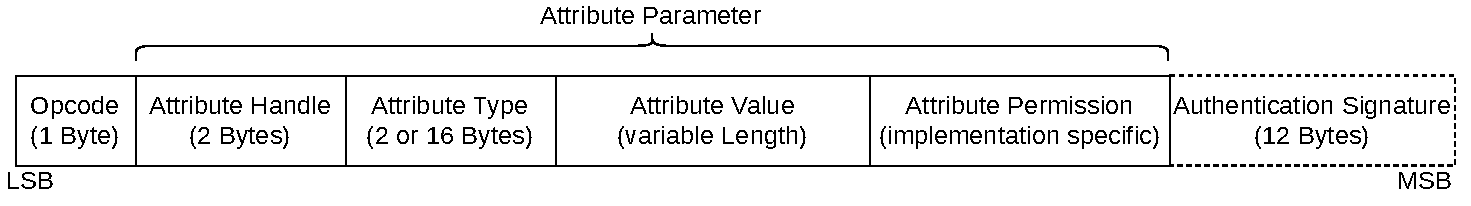
\includegraphics[width=0.9\textwidth]{graphics/att_pdu.pdf}
    \caption[(Generic) Attribute Protocol PDU]{(Generic) Attribute Protocol PDU; in Anlehnung an \cite{BtSpec4.0_fig_1888} und \cite{BtSpec4.0_fig_1889}}
    \label{fig: att pdu}
\end{figure}
% Quelle Spec 4.0 S. 1888 Figure 2.3 und S. 1889 Firgure 2.4

Der ein Byte lange Opcode sagt aus, ob die PDU entweder ein Request, eine Response, Notification, Indication oder Bestätigung ist, und enthält ein Flag für die Authentifizierung. Die Attributparameter unterteilen sich in zwei Byte für das Attribute Handle, zwei oder 16 Byte für den Attribute Type (die UUID), den Attributwert variabler Länge und die Attributberechtigungen, deren Länge von der Implementierung abhängig ist. Auf die Attributparameter folgt die 12 Byte lange Signatur für die Authentifizierung, falls gefordert. \cite{BtSpec4.0_1888-1889}
% QUELLE Spec 4.0 S. 1888 f.
\\\\

\begin{figure}{H}
    \centering
    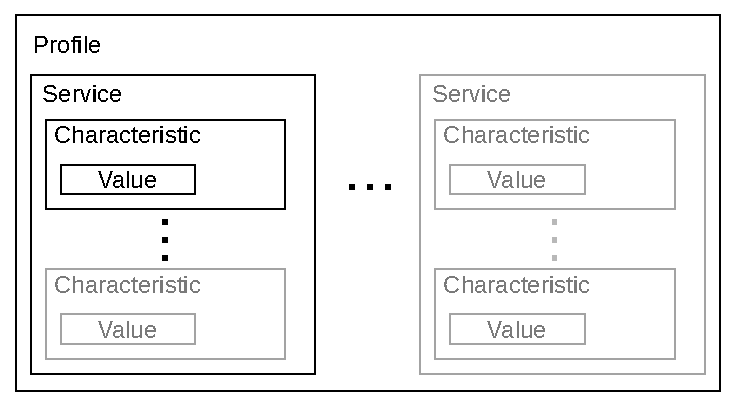
\includegraphics[width=0.9\textwidth]{graphics/gatt_hierarchie.pdf}
    \caption[]{\cite{BtSpec4.0_fig_1892}}
    \label{fig: gatt hierarchie}
\end{figure}
% Quelle Spec 4.0 S. 1892

GATT bildet eine Hierachie (siehe Abb. \ref{fig: gatt hierarchie}) bestehend aus den grundlegenden Elementen Profile, Service und Characteristic, die alle als Attribute definiert werden. An oberster Stelle befindet sich das Profile. Es enthält einen oder mehrere Services. Ein Service kann wiederum eine oder mehrere Characteristics enthalten, die sich aus Properties, einem Wert und Descriptors zusammensetzen.

		\subsubsection{Generic Access Profile}
			\label{sec: le gap}
			% TODO
Modes

Das Generic Access Profile (GAP) definiert verschiedene Rollen und Modi bzw. Prozeduren für Broadcasts und den Aufbau von Verbingungen.

Für LE existieren die vier Rollen: Broadcaster, Observer, Peripheral und Central. Ein Broadcaster ist aus Sicht des Link Layers (LL) ein Advertiser, da er verbindungslos Daten in Form von Advertising Events sendet. Der zugehörige Modus ist der Broadcast Mode. Diese Advertising Events können von Observern, die die Observation Procedure ausführen, empfangen werden, weswegen diese aus Sicht des LL als Scanner bezeichnet werden. Die Rolle Peripheral wird einem Gerät zugewiesen, wenn es den Aufbau eines LE Physical Link akzeptiert. Dabei nimmt es in Bezug auf den Link Layer die Rolle des Slave ein. Die Rolle Central wird einem Gerät zugewiesen, wenn dieses den Aufbau einer physischen Verbindung einleitet. Dabei nimmt es in Bezug auf den Link Layer die Rolle des Master ein. Ein Gerät kann mehrere Rollen zur selben Zeit einnehmen.
% TODO QUELLE Spec 4.0 S. 1638 f. 2.2.2 Roles when Operating over an LE Physical Channel
% TODO QUELLE Spec 4.0 S. 1695 f. 9.9.1 und 9.9.2

Jedes Gerät befindet sich entweder im Non-discoverable Mode, in dem es nicht von anderen Geräten entdeckt werden kann, oder im General Discoverable Mode bzw. im Limited Discoverable Mode, in denen es entdeckbar ist. Im Letzteren ist ein Gerät nur für eine bestimmte Dauer entdeckbar. Geräte, die andere Geräte entdecken sollen, müssen die General Discovery Procedure bzw. Limited Discovery Procedure ausführen.
% TODO QUELLE Spec 4.0 S. 1697 9.2 Discovery Modes And Procedures

Um Verbindungen und deren Aufbau zu steuern, gibt es mehrere Modi und Prozeduren, von denen einige in der Tabelle X zusammengefasst werden.
% TODO TABELLE VERWEIS

\begin{table}
    \begin{tabularx}{\textwidth}{|p{4.5cm}|X|}
    \hline
    \textbf{Modus/Prozedur} & \textbf{Beschreibung} \\
    \hline
    Non-connectable Mode & keine Verbindungen akzeptieren \\
    \hline
    Directed Connectable Mode & nur Verbindungen von bekannten Peer-Geräten akzeptieren, die die Auto oder General Connection Establishment Procedure ausführen \\
    \hline
    Undirected Connectable Mode & nur Verbindungen von Geräten akzeptieren, die die Auto oder General Connection Establishment Procedure ausführen \\
    \hline
    Auto Connection Establishment Procedure & Aufbau von Verbindungen zu Geräten, die in einem Connectable Mode sind und deren Adresse auf der Whitelist eingetragen ist \\
    \hline
    General Connection Establishment Procedure & Aufbau von Verbindungen zu bekannten Peer-Geräten, die in einem Connectable Mode sind \\
    \hline
    Connection Parameter Update Procedure & Peripheral oder Central kann Link-Layer-Parameter einer Verbindung ändern \\
    \hline
    \end{tabularx}
    \caption{Modi und Prozeduren für Verbindungen (Generic Access Profile)}
\end{table}
% TODO QUELLE Spec 4.0 S. 1704 - 1718 9.3 Connection Modes and Procedures

Zusätzlich verfügt GAP über Sicherheitsaspekte, die in Sektion X behandelt werden.
% TODO SEKTION VERWEIS BLE Sicherheit

		\subsubsection{Security Manager}
			\label{sec: le sm}
			Der Security Manager (SM) bzw. das Security Manager Protocol (SMP) ist dafür zuständig eine sichere Verbindung zwischen zwei Geräten (Master und Slave) aufzubauen. Dies umfasst im Wesentlichen das Pairing, welches zur Authentifizierung und Generierung eines Schlüssels dient, und die Verteilung von Schlüsseln. Entsprechend der Abb. \ref{fig: smp in bt} lässt sich der Security Manager bzw. das SMP in die BLE-Architektur einordnen.

\begin{figure}[H]
    \centering
    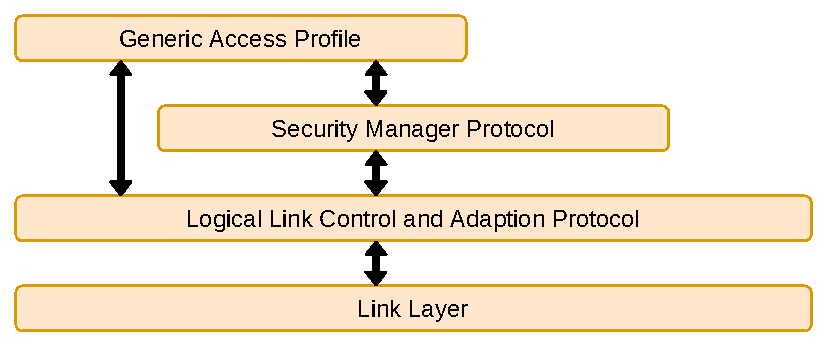
\includegraphics[width=0.8\textwidth]{graphics/smp_in_bt.pdf}
    \caption[Beziehungen des Security Managers zu anderen Host-Komponenten]{Beziehungen des Security Managers zu anderen Host-Komponenten; in Anlehnung an \cite{BtSpec4.0_fig_1958}}
    \label{fig: smp in bt}
\end{figure}
% QUELLE Spec 4.0 S. 1958

Um mit dem Link Layer zu interagieren, nutzt der SM einen L2CAP Channel mit einer festgelegten CID. Zudem kann er mit GAP direkt kommunizieren.
\\\\
Das Pairing lässt sich in drei Phasen aufteilen. Phase 1 und 2 dienen der Generierung eines Schlüssels, den beide Geräte zur Verschlüsselung und Authentifizierung im Link Layer nutzen. Dafür wird der Cipher Block Chaining - Message Authentication Code (CCM) Mode in Verbindung mit dem Advanced Encryption Standard (AES), genauer dem AES-128 Block Cipher, genutzt \cite{BtSpec4.0_2285}.
% QUELLE Spec. 4.0 S. 2285, 1 ENCRYPTION AND AUTHENTICATION OVERVIEW

\paragraph{Pairing: Phase 1} \mbox{} \vspace{0.2cm} \\
Die erste Phase ist der Pairing Feature Exchange, bei dem die beiden Geräte ihre für den Nutzer zugänglichen Ein- und Ausgabemöglichkeiten (IO Capabilities) austauschen. Die Tabellen \ref{tab: i caps geraet} und \ref{tab: o caps geraet} 
listen die entsprechenden Bezeichnungen dieser Möglichkeiten auf.
\\\\

\begin{table}[H]
    \begin{tabularx}{\textwidth}{|l|X|}
    \hline
    \textbf{Eingabemöglichkeit} & \textbf{Beschreibung} \\
    \hline
    Keine Eingabe & Gerät kann keine Eingaben entgegennehmen \\
    \hline
    Ja / Nein & Gerät kann zwei verschiedene Eingaben verarbeiten, die der Bedeutung Ja bzw. Nein zugewiesen werden können (bspw. zwei Tasten) \\
    \hline
    Tastatur & Eingabe der Ziffern 0 bis 9 möglich und die Möglichkeit Ja und Nein einzugeben \\
    \hline
    \end{tabularx}
    \caption[Eingabemöglichkeiten eines Gerätes]{Eingabemöglichkeiten eines Gerätes \cite{BtSpec4.0_1965}}
    \label{tab: i caps geraet}
\end{table}

\begin{table}[H]
    \begin{tabularx}{\textwidth}{|l|X|}
    \hline
    \textbf{Ausgabemöglichkeiten} & \textbf{Beschreibung} \\
    \hline
    Keine Ausgabe & Gerät kann keine 6-stellige Dezimalzahl dem Nutzer anzeigen bzw. kommunizieren \\
    \hline
    Numerische Ausgabe & Gerät kann eine 6-stellige Dezimalzahl dem Nutzer anzeigen bzw. kommunizieren \\
    \hline
    \end{tabularx}
    \caption[Ausgabemöglichkeiten eines Gerätes]{Ausgabemöglichkeiten eines Gerätes \cite{BtSpec4.0_1965_b}}
    \label{tab: o caps geraet}
\end{table}
% QUELLE für Tabellen: Spec 4.0 S. 1965 Table 2.1 und Table 2.2

Desweiteren tauschen die Geräte in der ersten Phase Informationen darüber aus, ob eine Authentifizierung zum Schutz vor einem Man-In-The-Middle-Angriff nötig ist (MITM Flag), und ob Daten für die Authentifizierung über die Pairing-Methode Out Of Band (OOB), d.h. mittels einer anderen Technologie (z.B. Near Field Communication), übertragen werden können (OOB Flag). Außerdem werden die minimalen und maximalen Größen für die Schlüssel ausgetauscht, die sich in 8 Bit großen Schritten zwischen 56 Bit (7 Byte) und 128 Bit (16 Byte) befinden. Dabei wird der kleinere Wert beider maximaler Größen übernommen. Falls die beiden Spannen sich nicht schneiden, wird das Pairing abgebrochen.

\paragraph{Pairing: Phase 2} \mbox{} \vspace{0.2cm} \\
Anhand der ausgetauschten Informationen aus der ersten Phase wird in der zweiten Phase entschieden, welche der folgenden Methoden zur Generierung des Short Term Key (STK) bzw. Long Term Key (LTK) zu verwenden ist:

\begin{itemize}
    \item{Numeric Comparison (für LE erst ab Bluetooth-Version 4.2)}
    \item{Just Works}
    \item{Out of Band (OOB)}
    \item{Passkey Entry}
\end{itemize}

Da das Pairing (speziell Phase 2) für LE in der Bluetooth-Version 4.0 funktionale Unterschiede zum Pairing für LE ab Version 4.2 aufweist, wird das Pairing für LE in Version 4.0 als \textbf{LE Legacy Pairing} und das Pairing für LE ab Version 4.2 als \textbf{LE Secure Connections Pairing} bezeichnet. Aus Sicht des Nutzers sind diese jedoch gleich und jede Bluetooth-Version, die LE unterstützt, unterstützt das LE Legacy Pairing. Im Gegensatz zum LE Secure Connections Pairing bietet LE Legacy Pairing für die Methoden Just Works und Passkey Entry keinen Schutz vor passivem Abhören während des Pairings, da LE Secure Connections Elliptic Curve Diffie-Hellman (ECDH) für den Schlüsselaustausch nutzt und LE Legacy Pairing nicht. \cite{BtSpec4.2_248}
% QUELLE Spec 4.2 S. 248 5.4.1 Association Models
\\\\
Haben beide Geräte OOB-Authentifizierungsdaten für das LE Legacy Pairing, wird unabhängig von der jeweiligen MITM-Flag die Methode OOB gewählt. In LE Secure Connections Pairing wird ebenso verfahren, nur dass hier nicht die OOB-Flag beider Geräte gesetzt sein müssen (aber können), da eine gesetzte OOB-Flag genügt. Ist die MITM-Flag beider Geräte nicht gesetzt, wird die Methode Just Works ausgeführt. Anderenfalls werden die Ein- und Ausgabemöglichkeiten der Geräte für die Wahl der Methode einbezogen entsprechend \cite{BtSpec4.2_tab_2302-2303}.
% Verweis TABELLE Spec 4.2 S. 2302 f., Table 2.8

\subparagraph{Pairing Methoden} \mbox{} \vspace{0.2cm} \\
Bei der \textbf{Numeric Comparison} wird dem Nutzer auf beiden Geräten jeweils eine zufällig generierte sechsstellige Dezimalzahl angezeigt. Diese muss der Nutzer vergleichen und im Falle der Übereinstimmung auf beiden Geräten bestätigen oder anderenfalls ablehnen. Somit kann der Nutzer unabhängig von der Namensgegebung der Geräte sicherstellen, die richtigen Geräte ausgewählt zu haben. Zudem bietet diese Methode Schutz vor MITM-Angriffen. Außenstehende, die Kenntnis über diese Zahl gewonnen haben, können laut \cite{BtSpec4.2_244-245} damit keinen Vorteil zur Entschlüsselung der zwischen den beiden Geräten ausgetauschten Daten erlangen, da die Zahl nicht als Eingabe zur Generierung eines Schlüssels verwendet wird.
% QUELLE VERWEIS Sepc 4.2 S. 244 f. 5.2.4.1 Numeric Comparison

\textbf{Just Works} basiert auf der Funktionsweise von Numeric Comparison mit dem Unterschied, dass hier dem Nutzer keine sechsstellige Dezimalzahl ausgegeben wird und er die Verbindung nur bestätigen muss. Dadurch bietet Just Works keinen Schutz vor MITM-Angriffen, aber einen Schutz gegen passives Abhören (außer für LE Legacy Pairing). \cite{BtSpec4.2_245}
% QUELLE Spec 4.2 S.245 5.2.4.2 Just Works

\textbf{Out of Band} ist die Nutzung einer anderen Technologie (z.B. Near Field Communication), um Geräte zu entdecken oder um kryptographische Informationen für den Pairing-Prozess auszutauschen. Dabei sollte die Technologie Schutz vor MITM-Angriffen bieten. \cite{BtSpec4.2_246}
% QUELLE Spec 4.2 S. 246 5.2.4.3 Out of Band

Die Methode \textbf{Passkey Entry} definiert, dass ein Gerät die zufällig generierte sechstellige Dezimalzahl ausgibt und der Nutzer diese auf dem anderen Gerät eingeben muss. Ein Schutz gegen MITM-Angriffe existiert, da diese nur mit einer Wahrscheinlichtkeit von 0,000001 für jede Durchführung der Methode möglich sind. Schutz gegen passives Abhören bietet Passkey Entry nur in LE Secure Connections Pairing und nicht in LE Legacy Pairing. \cite{BtSpec4.2_246-247} \cite{BtSpec4.2_2304}
% QUELLE Spec 4.2 S. 246 f. 5.2.4.4 Passkey Entry
% QUELLE Spec. 4.2 S. 2304 2.3.5.3 LE Legacy Pairing - Passkey Entry

\subparagraph{LE Legacy Pairing: Schlüssel und deren Generierung} \mbox{} \vspace{0.2cm} \\
Beim LE Legacy Pairing zweier Geräte generieren beide einen 128 Bit langen Temporary Key (TK), der bei der Authentifizierung genutzt wird, um den STK zu generieren und die Verbindung zu verschlüsseln. In Just Works wird der TK auf null gesetzt. Bei der Methode Passkey Entry ist der TK die besagte zufällig generierte sechstellige Dezimalzahl, die bereits mit 20 Bit dargestellt werden kann, weswegen die restlichen Bit des TK auf null gesetzt werden müssen. Dagegen kann bei OOB auf diese Einschränkung verzichtet werden, wodurch der TK wahrhaftig eine Länge von 128 Bit besitzt.

Das Gerät, welches das Pairing einleitet (Master), generiert eine zufällige 128 Bit große Nummer \textit{Mrand} und ermittelt den 128 Bit großen Bestätigungswert \textit{Mconfirm} mit der Confirm Value Generation Function c1 \cite{BtSpec4.2_2288}. 
% QUELLE Spec. 4.2 S. 2288 2.2.3 Confirm value generation function c1 for LE Legacy Pairing
Zur Berechnung von \textit{Mconfirm} erhält die Funktion c1 folgende Eingabewerte entsprechend Gl. \ref{eq: mconfirm} \cite{BtSpec4.2_2305-2306}.

\begin{equation}
\begin{split}
    \text{Mconfirm} = \text{c1}(& \text{TK, Mrand,} \\
    & \text{Pairing Request Command, Pairing Response Command,} \\
    & \text{Adresstyp des Masters, Adresse des Masters,} \\
    & \text{Adresstyp des Slaves, Adresse des Slaves}) \\
\end{split}
    \label{eq: mconfirm}
\end{equation}

Ebenso führt das antwortende Gerät (Slave) diese Schritte durch, wobei \textit{Mrand} als \textit{Srand} bezeichnet wird und \textit{Mconfirm} als \textit{Sconfirm}. Die Eingabewerte der Funktion c1 zur Berechnung von \textit{Sconfirm}sind demnach analog zu denen von \textit{Mconfirm}. Danach findet entsprechend Abb. \ref{fig: austausch vor stk generierung} folgender Austausch statt.

\begin{figure}[H]
    \centering
    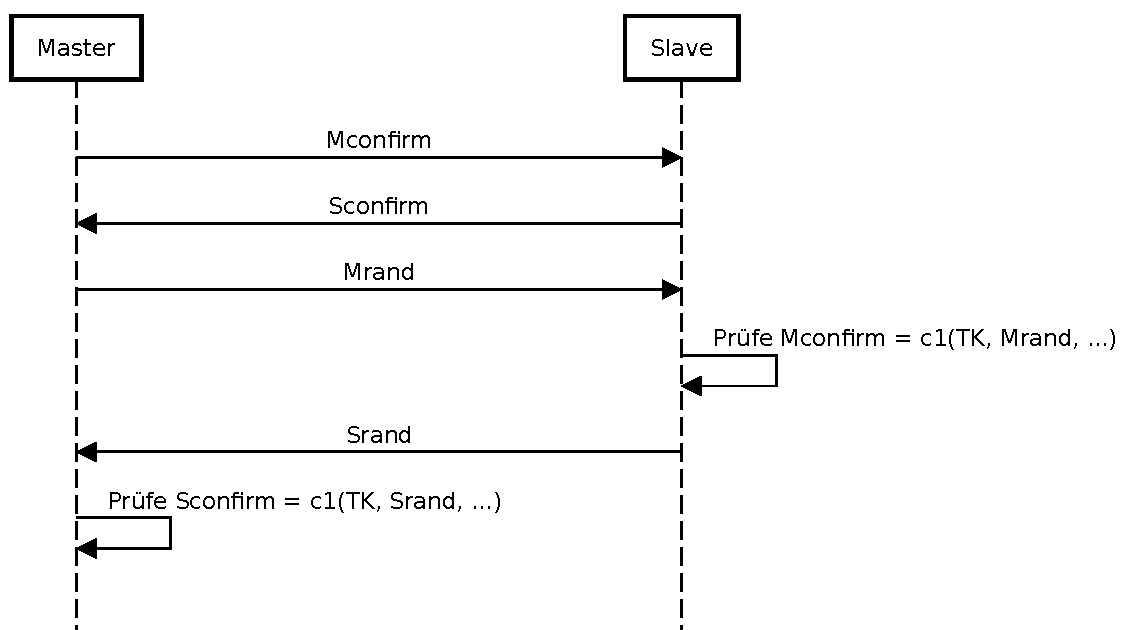
\includegraphics[width=0.9\textwidth]{graphics/austausch_vor_stk_generierung.pdf}
    \caption[Austausch von \textit{Mconfirm}, \textit{Sconfirm}, \textit{Mrand} und \textit{Srand} zwischen Master und Slave]{Austausch von \textit{Mconfirm}, \textit{Sconfirm}, \textit{Mrand} und \textit{Srand} zwischen Master und Slave \cite{BtSpec4.2_2305-2306}}
    \label{fig: austausch vor stk generierung}
\end{figure}

Master und Slave tauschen \textit{Mconfirm} und \textit{Sconfirm} aus. Danach überträgt der Master \textit{Mrand}, damit der Slave \textit{Mconfirm} entsprechend Gl. \ref{eq: mconfirm} berechnen und so den empfangenen \textit{Mconfirm} verifizieren kann. Nach einer erfolgreichen Prüfung von \textit{Mconfirm} überträgt der Slave \textit{Srand}, damit der Master \textit{Sconfirm} analog zu Gl. \ref{eq: mconfirm} berechnen und somit den empfangenen \textit{Sconfirm} verifizieren kann. Wenn einer der Bestätigungswerte (\textit{Mconfirm}, \textit{Sconfirm}) nicht erfolgreich verifiziert wird, wird die Verbindung sofort beendet.
\\\\
Anschließend wird der STK mit der Funktion s1 \cite{BtSpec4.2_2290} 
% QUELLE verweis auf Spec 4.2 S. 2290 2.2.4 Key generation function s1 for LE Legacy Pairing
entsprechend Gl \ref{eq: stk} \cite{BtSpec4.2_2305-2306} berechnet.

\begin{equation}
    \text{STK} = \text{s1}(\text{TK, Srand, Mrand})
    \label{eq: stk}
\end{equation}

Demnach kann bei der Methode Passkey Entry kein ausreichender Schutz gegen passives Abhören geboten werden, da der TK nur wenig mögliche Werte annehmen kann. Ist die vereinbarte Schlüsselgröße kleiner als 128 Bit, werden die überschüssigen Bit beginnend bei dem Bit mit dem höchsten Stellenwert auf null gesetzt. Der STK wird nun zur Verschlüsselung der Verbindung genutzt. \cite{BtSpec4.2_2305-2306}
% QUELLE Spec. 4.2 S. 2305 f. 2.3.5.5 LE Legacy Pairing Phase 2

\subparagraph{LE Secure Connections Pairing: Schlüssel und deren Generierung} \mbox{} \vspace{0.2cm} \\
Beim LE Secure Connections Pairing wird ein Long Term Key (LTK) erstellt. Zuvor erstellen beide Geräte jeweils ein ECDH-Schlüsselpaar (PK - Public Key, SK - Private Key) und tauschen ihre Public Keys aus. Danach berechnet jedes Gerät den Diffie-Hellman-Schlüssel aus seinem Private Key und dem Public Key des Anderen. Durch den Diffie-Hellman-Schlüssel kennen beide Parteien ein gemeinsames Geheimnis, mit dem sie den weiteren Datenaustausch zur Authentifizierung verschlüsseln können. Die Authentifizierung ist notwendig, da der ECDH-Schlüsselaustausch zwar resistent gegen passives Abhören ist, jedoch nicht gegen MITM-Angriffe. \cite{BtSpec4.2_2307}
% QUELLE Spec. 4.2 S. 2307 2.3.5.6.1 Public Key Exchange

Diese Authentifizierung wird mit den Pairing Methoden Numeric Comparison, Just Works, OOB und Passkey Entry ermöglicht. Jedoch unterscheiden diese sich aus funktionaler Sicht (nicht aus Nutzersicht) zum LE Legacy Pairing durch komplexere Verfahren. Letztendlich lässt sich für die vier Pairing-Methoden Folgendes zusammenfassen. Numeric Comparison signalisiert dem Nutzer mit einer Wahrscheinlichkeit von 0,999999 einen stattfindenden MITM-Angriff \cite{BtSpec4.2_2309}. 
% QUELLE Spec. 4.2 S. 2309, 2.3.5.6.2 Authentication Stage 1 – Just Works or Numeric Comparison
Just Works bietet keinen Schutz vor einem MITM-Angriff \cite{BtSpec4.2_245}. 
% QUELLE Spec. 4.2 S. 245, 5.2.4.2 Just Works
Ein MITM-Angriff während des Passkey Entry gelingt nur mit einer Wahrscheinlichkeit von 0,000001 \cite{BtSpec4.2_2311}. 
% QUELLE Spec. 4.2 S. 2311, 2.3.5.6.3 Authentication Stage 1 – Passkey Entry
Wie anfällig OOB für Angriffe ist hängt von der verwendeten OOB-Technologie ab \cite{BtSpec4.2_2312-2313}.
% QUELLE Spec. 4.2 S. 2312 f., 2.3.5.6.4 Authentication Stage 1 – Out of Band

Nach der Ausführung einer Pairing-Methode wird der LTK als Teilergebnis der Funktion f5 \cite{BtSpec4.2_2292-2293} 
% QUELLE Spec. 4.2 S. 2292 f., 2.2.7 LE Secure Connections Key Generation Function f5
mit den Eingabewerten Diffie-Hellman-Key, ein Nonce des Masters, ein Nonce des Slaves und der Adresse des Masters und Slaves ermittelt \cite{BtSpec4.2_2314}.
% QUELLE Spec. 4.2 S. 2314, 2.3.5.6.5 Authentication Stage 2 and Long Term Key Calculation

\paragraph{Pairing: Phase 3} \mbox{} \vspace{0.2cm} \\
Wurde der STK bzw. LTK generiert, wird dieser genutzt, um die Verbindung zu verschlüsseln. Nun können in der dritten Phase transportspezifische Schlüssel ausgetauscht werden. Z.B. wird der Identity Resolving Key (IRK) zur Generierung und Auflösung von zufälligen Adressen verwendet und der Connection Signature Resolving Key (CSRK) zur Signatur von Daten und Überprüfung von Signaturen.

% Für Numeric Comparison und Just Works wird entsprechend Abb. X fortgefahren.
% % TODO BILD VERWEIS

% \begin{figure}[hbt!]
%     \centering
%     \inlcudegraphics[width=0.5\linewidth]{graphics/LE_Secure_Connections_Pairing_Numeric_Comparison_Just_Works.svg}
%     \caption{}
% \end{figure}

% Der zu Beginn zufällig generierte Nonce (N\textunderscore a bzw. N\textunderscore b) mit einer Länge von 128 Bit wird für jeden Durchlauf neu erzeugt und schützt vor Replay-Angriffen. Für die Berechnung der Bestätigung C\textunderscore b wird die Einwegfunktion f4 [X] genutzt. 
% % TODO QUELLE Spec. 4.2 S. 2291 2.2.6 LE Secure Connections Confirm Value Generation Function f4
% Mittels der Funktion g2 [X] 
% % TODO QUELLE Spec 4.2 S. 2295 2.2.9 LE Secure Connections Numeric Comparison Value Generation Function g2
% werden die Dezimalzahlen D\textunderscore a und D\textunderscore b berechnet. Darauf werden diese dem Nutzer auf den Geräten ausgegeben und dieser muss deren Gleichheit bestätigen. Wird anstatt Numeric Comparison die Methode Just Works ausgeführt, dann werden D\textunderscore a und D\textunderscore b nicht berechnet und folglich nicht dem Nutzer gezeigt. Sollte ein Fehler auftreten wird das Protokoll abgebrochen und kann neu gestartet werden.

% Beim vorherigen ECDH-Schlüsselaustausch, kann ein MITM-Angriff angewandt werden. Eine einfache Variante, die keine Informationen der beiden angegriffenen Geräte zwischen diesen austauscht sondern mit diesen jeweils separat die Methode Numeric Comparison durchführt, endet darin, dass dem angegriffenem Nutzer mit einer Wahrscheinlichkeit von 0,999999 auf dessen Geräten zwei verschiedene Dezimalzahlen angezeigt werden. Eine andere Variante wäre aus Sicht des Angreifenden den Verkehr bestehend aus der Bestätigung C\textunderscore b, dem Nonce N\textunderscore a und N\textunderscore b nur weiterzuleiten. Jedoch wird der Master bei der Überprüfung der Bestätigung C\textunderscore b feststellen, dass diese nicht mit seinem Public Key PK\textunderscore a erstellt wurde, was zum Abbruch führt.\\\\
% % TODO QUELLE Spec. 4.2 S. 2308 f. 2.3.5.6.2 Authentication Stage 1 – Just Works or Numeric Comparison
% Passkey Entry
% OOB

	\subsection{Sicherheit}
		\label{sec: le security}
		Obwohl Bluetooth LE mit dem Privacy Feature und dem Security Manager (vor allem ab Bluetooth 4.2) einige Optionen für eine sichere Infrastruktur bietet, bleiben Probleme offen, die betrachtet werden müssen.
\\\\
Ein erfolgreicher Angriff auf zwei Geräte, die mittels BLE verschlüsselt kommunizieren, in Form von passivem Abhören oder eines MITM-Angriffs kann beim Aufbau einer Verbindung, also dem Pairing (siehe Sektion \ref{sec: le sm}), auftreten, da hier die Schlüssel ausgetauscht werden. In Tabelle \ref{tab: le sicherheit zusammenfassung}
wird dargestellt welchen Schutz die Pairing-Methoden des LE Legacy Pairing und des LE Secure Connections Pairing gegen passives Abhören und MITM-Angriffe bieten.

\begin{table}
    \begin{tabularx}{\textwidth}{|p{2.8cm}|p{2cm}|p{3cm}|p{2cm}|p{3cm}|}
        \hline
        & \multicolumn{2}{X|}{\textbf{Schutz gegen Passives Abhören}} & \multicolumn{2}{X|}{\textbf{Schutz gegen MITM-Angriff}} \\
        & \textbf{LE Legacy} & \textbf{LE Secure Connections} & \textbf{LE Legacy} & \textbf{LE Secure Connections} \\
        \hline
        \textbf{Numeric Comparison} & - & Ja & - & Ja \cite{BtSpec4.2_2309} \\
        \hline
        \textbf{Just Works} & Nein \cite{BtSpec4.2_2304_b} & Ja \cite{BtSpec4.2_245} & Nein \cite{BtSpec4.2_2304_b} & Nein \cite{BtSpec4.2_245} \\
        \hline
        \textbf{Out of Band} & \multicolumn{4}{|l|}{abhängig von OOB-Technologie \cite{BtSpec4.2_2305} \cite{BtSpec4.2_2312-2313}} \\
        \hline
        \textbf{Passkey Entry} & Nein \cite{BtSpec4.2_2304} & Ja & Ja \cite{BtSpec4.2_2304} & Ja \cite{BtSpec4.2_2311}\\
        \hline
    \end{tabularx}
    \caption[Schutz durch Pairing-Methoden vor passivem Abhören und MITM]{Schutz durch Pairing-Methoden vor passivem Abhören und MITM-Angriffen; Der Bindestrich symbolisiert, dass diese Methode nicht verfügbar ist. LE Secure Connections ist aufgrund des ECDH-Schlüsselaustausches \cite{BtSpec4.2_2307} generell vor passivem Abhören geschützt.}
    \label{tab: le sicherheit zusammenfassung}
\end{table}
% QUELLE Spec. 4.2 S. 2304, 2.3.5.2 LE Legacy Pairing - Just Works
% QUELLE Spec. 4.2 S. 245, 5.2.4.2 Just Works
% QUELLE Spec. 4.2 S. 2305, 2.3.5.4 Out of Band
% QUELLE Spec. 4.2 S. 2312, 2.3.5.6.4 Authentication Stage 1 – Out of Band
% QUELLE Spec. 4.2 S. 2304, 2.3.5.3 LE Legacy Pairing - Passkey Entry
% QUELLE Spec. 4.2 S. 2311, 2.3.5.6.3 Authentication Stage 1 – Passkey Entry

Dabei ist zu beachten, dass die Methode Numeric Comparison dem Nutzer mit einer Wahrscheinlichkeit von 0,999999 einen stattfindenden MITM-Angriff signalisiert \cite{BtSpec4.2_2309}, bevor dieser das Pairing fortsetzt, und dass die Methode Passkey Entry nur mit einer Wahrscheinlichkeit von 0,000001 anfällig für einen MITM-Angriff ist \cite{BtSpec4.2_2304} \cite{BtSpec4.2_2311}. Die Methode OOB des LE Legacy Pairing ist bei einer sicheren OOB-Technologie ebenfalls mit einer Wahrscheinlichkeit von 0,000001 oder kleiner (je nach Schlüsselgröße) anfällig gegen MITM-Angriffe \cite{BtSpec4.2_2305}.
% QUELLE Spec. 4.2 S. 2309, 2.3.5.6.2 Authentication Stage 1 – Just Works or Numeric Comparison
% QUELLE Spec. 4.2 S. 2304, 2.3.5.3 LE Legacy Pairing - Passkey Entry
% QUELLE Spec. 4.2 S. 2311, 2.3.5.6.3 Authentication Stage 1 – Passkey Entry
% QUELLE Spec. 4.2 S. 2305, 2.3.5.4 Out of Band

Obwohl die Methoden Numeric Comparison und Passkey Entry des LE Secure Connections Pairing eine beachtliche Sicherheit bieten, ist laut den Bluetooth-Spezifikationen 4.0 bis 5.2 jede dieser Bluetooth-Versionen in der Lage das LE Legacy Pairing auszuführen \cite{BtSpec4.2_248_b} \cite{BtSpec5.2_277}, welches wiederum anfälliger ist (OOB ausgenommen). 
% QUELLE Spec. 4.2 S. 248, 5.4 LE SECURITY
% QUELLE Spec. 5.2 S. 277, 5.4 LE SECURITY
Vermutlich kann dies durch die letztendlichen Entwickler einer Bluetooth-Software bzw. -Hardware oder durch den Anwender selbst eingeschränkt werden. Falls dies nicht umgesetzt wird, stellt die Möglichkeit einer Rückstufung auf LE Legacy Pairing ein Sicherheitsrisiko dar.

Dabei sei zu erwähnen, dass jede Methode bestimmte Möglichkeiten zur Ein- und Ausgabe von den zu verwendenten Geräten voraussetzt. Ist es für den Anwender nicht möglich diese Voraussetzungen in den Geräten zu implementieren, kann BLE selbst keine Schutz bieten.
\\\\
Ein weiteres Problem ist die Sicherheit auf der Anwendungsebene. Unterstützt ein System weitere Anwendungen, auf die der Anwender keinen Zugriff hat, könnte es möglich sein, dass eine solche fremde Anwendung auf Daten zugreifen kann, die nur für die Anwendung des Anwenders bestimmt sind. Die Möglichkeit dazu besteht, da BLE zu übertragende Daten innerhalb des Controllers auf der Ebene des Link Layer verschlüsselt \cite{BtSpec4.0_196} \cite{BtSpec4.0_2285}. 
% QUELLE Spec. 4.0 S. 196, 5.2.3 Encryption
% QUELLE Spec. 4.0 S. 2285, 1 ENCRYPTION AND AUTHENTICATION OVERVIEW

Ein Beispiel für ein solches System ist das Betriebssystem Android von der Open Handset Alliance. Auf Androids Webpräsenz für BLE wird darauf hingewiesen, dass BLE keine Sicherheit auf Anwendungsebene liefert: "When a user pairs their device with another device using BLE, the data that's communicated between the two devices is accessible to all apps on the user's device" \cite{AndroidAppLayerSec}.
% QUELLE ZITAT https://developer.android.com/guide/topics/connectivity/bluetooth-le Bluetooth low energy -> Caution

Den Beweis dafür, dass Daten, die durch BLE über den Link Layer verschlüsselt oder unverschlüsselt übertragen werden, von anderen Apps ausgelesen werden können, liefert eine Studie der Royal Holloway University of London \cite{RoyalHollowayUniversity}. Diese zeigt, wie innerhalb des Android Betriebssystems eine fremde Anwendung Daten über das Protokoll ATT bzw. GATT 
empfangen kann, die theoretisch für eine andere Anwendung bestimmt sind.
% QUELLE
% A Study of the Feasibility of Co-located App Attacks against BLE and a Large-Scale Analysis of the Current Application-Layer Security LandscapePallavi Sivakumaran and Jorge Blasco, Royal Holloway University of London
% PDF S. 4 - 6
% https://www.usenix.org/conference/usenixsecurity19/presentation/sivakumaran 


% TODOOPT Angriff: BLESA, für GATT relevant

\newpage
\section{Infrastruktur}
	\label{sec: infra allg}
	Die Infrastruktur beschreibt eine allgemeine Lösung, um eine sichere Kommunikation mittels Bluetooth Low Energy (BLE) zwischen einem Mikrocontroller und einem Smartphone zu gewährleisten. Bis auf den Fakt, dass ein Mikrocontroller und ein Smartphone über BLE miteinander kommunizieren, sind die spezifischen Systeme der beiden Kommunikationsparteien nicht vorgegeben. Dennoch ist die Lösung universell einsetzbar, solange jedes System über ein Bluetooth"=Modul (mind. der Bluetooth"=Version 4.0) verfügt. Da das Protokoll \textit{Transport Layer Security} (TLS) ein wesentlicher Bestandteil des Lösungsansatzes ist, müssen die Systeme eine Software"=Bibliothek für TLS unterstützen. Somit ist die Infrastruktur unabhängig von dem in der Sektion \ref{sec: einleitung} beschriebenen Projekt SteigtUM.
\\\\
Da das Ziel dieser Infrastruktur die sichere Datenübertragung zwischen zwei Kommunikationsparteien ist, sollte diesbezüglich "`Sicherheit"' definiert werden. Nach \cite{Bless2005_19-20} werden mehrere Sicherheitsziele definiert um ein sicheres Netzwerk zu schaffen. Daraus ergeben sich die für diese Infrastruktur wesentlichen Sicherheitsziele der Vertraulichkeit, Datenintegrität und Authentizität.
% QUELLE S. 19 https://books.google.de/books?id=-fciBAAAQBAJ&lpg=PA2&ots=YPh7AK5_WJ&dq=sichere%20Daten%C3%BCbertragung&lr&pg=PA19#v=onepage&q&f=false

Vertraulichkeit bedeutet, dass "`Übertragene Daten [...] nur berechtigten Instanzen zugänglich sein [sollen], d.h. keine unbefugte dritte Partei soll an den Inhalt von übertragenen Nachrichten gelangen können"' \cite{Bless2005_19}.
% QUELLE ZITAT
Die Datenintegrität trägt folgende Bedeutung. "`Für den Empfänger muss eindeutig erkennbar sein, ob Daten während ihrer Übertragung unbefugt geändert wurden"' \cite{Bless2005_19}.
% QUELLE ZITAT 
Authentizität teilt sich in zwei Punkte auf. Zum einen soll "`eine Instanz [...] einer anderen ihre Identität zweifelsfrei nachweisen können (Identitätsnachweis bzw. Authentifizierung der Instanz)"' \cite{Bless2005_19}. 
% QUELLE ZITAT
Zum anderen "`soll überprüft werden können, ob eine Nachricht von einer bestimmten Instanz stammt (Authentizität der Daten)"' \cite{Bless2005_19}.
% QUELLE ZITAT

	\subsection{Topologie}
		\label{sec: infra topologie}
		Die Topologie der Infrastruktur beschränkt sich auf das Minimum an Kommunikationsparteien und ist unabhängig von der Anwendung.\\

% TODO BILD topologie infratruktur mikrocontroller, smartphone, CA

Dem Thema zufolge sollen ein Mikrocontroller und ein Smartphone sicher Daten austauschen. Um dies zu bewerkstelligen, wird über den Transport der Daten durch Bluetooth Low Energy (BLE) das Verschlüsselungsprotokoll TLS verwendet (siehe Sektion X). 
% TODO SEKTION VERWEIS Infrakstruktur->Sicherheit
Dementsprechend ist, wie in Abbildung X zu sehen
% TODO BILD VERWEIS topologie infrastruktur mikrocontroller, smartphone, CA
, neben dem Mikrocontroller und dem Smartphone eine Zertifizierungsstelle notwendig. In welcher Form diese auftritt ist von der Anwendung abhängig.

Für einen seriösen Anwendungsfall sollte die Zertifizierungsstelle evtl. in Form eines Servers existieren, der dem Mikrocontroller und Smartphone in regelmäßigen Abständen (z.B. jährlich) jeweils ein Zertifikat ausstellt. Mit diesen Zertifikaten und der Kenntnis über das Root-Zertifikat können Mikrocontroller und Smartphone sich gegenseitig authentifizieren und somit die Grundlage für eine sichere Kommunikation bilden.

Beispielsweise könnte es für einen privaten Anwendungsfall ausreichend sein, die Zertifizierungsstelle nicht als dauerhaft betriebenen Server darzustellen, sondern lediglich ein Root-Zertifikat zu erstellen und mit diesem dem Mikrocontroller und Smartphone jeweils ein digitales Zertifikat auszustellen.

Die Rolle der Partei, die die Zertifikate für Mikrocontroller und Smartphone austellt muss nicht zwingend eine Zertifizierungsstelle sein, sondern könnte auch eine Entität sein, der von einer Zertifizierungsstelle ein Zwischenzertifikat ausgestellt wurde.

	\subsection{Transport}
		\label{sec: infra transport}
		Eine der grundlegendsten Bedingungen dieser Arbeit ist, dass BLE als Technologie zum Übertragen der Daten zwischen Smartphone und Mikrocontroller genutzt werden soll. Demnach stellt sich die Frage nach einem geeigneten Transport der Daten innerhalb der BLE"=Architektur.
\\\\
Es existieren mehrere Referenzmodelle für die Kommunikation innerhalb von Rechnernetzen. Geläufig sind das TCP/IP"=Referenzmodell (Transport Control Protocol / Internet Protocol), das OSI"=Referenzmodell (Open Systems Interconnection) und ein hybrides Referenzmodell aus diesen beiden. Alle drei legen sich auf unterschiedliche Anzahlen von Schichten fest, von denen sich einige gleichen oder ähneln und andere nicht. Die Eigenschaften der Transportschicht sind bei den drei Referenzmodellen identisch. Die zu übertragenden Daten der darüberliegenden Anwendungsschicht werden in Segmente aufgeteilt und von einem Endpunkt über die niedrigeren Schichten zum anderen Endpunkt gesendet. Auf Empfängerseite erhält die Transportentität diese Segmente, setzt sie wiederzusammen und übergibt sie der zugehörigen Anwendung, die mithilfe von Ports identifiziert wird. Demnach kann die Transportschicht eine verbindungslose oder verbindungsorientierte Datenübertragung unterstützen, wobei die verbindungsorientierte Übertragung Flusskontrolle, verlustfreie Übertragung und die korrekte Reihenfolge der Segmente unterstützen kann. \cite{Baun2019_36-40}
% QUELLE https://katalog.ub.tu-freiberg.de/Record/0-1666728691, https://link.springer.com/book/10.1007%2F978-3-658-26356-0, Computer Networks / Computernetze von Christian Baun, S. 39 Transportschicht
\\\\
Die BLE"=Architektur lässt sich entsprechend der Abb. \ref{fig: hyb referenzmodell ble} am besten dem hybriden Referenzmodell zuordnen, da dieses im Gegensatz zum OSI-Referenzmodell die Anwendungsschicht nicht in drei weitere Schichten unterteilt und abgesehen von dieser Differenz dem OSI-Referenzmodell gleicht.

\begin{figure}[H]
    \centering
    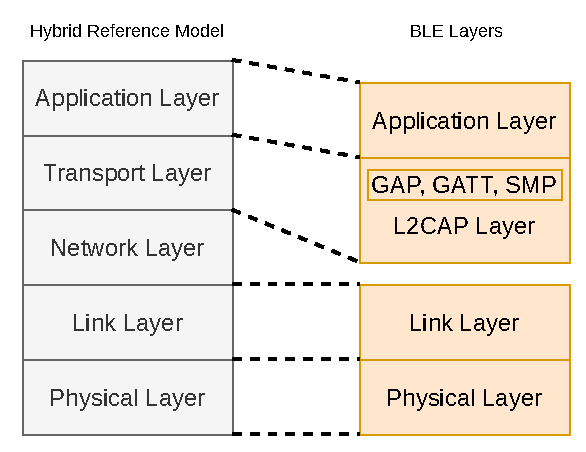
\includegraphics[width=0.55\textwidth]{graphics/hybr_referenzmodell_zu_ble.pdf}
    \caption[Zuordnung der BLE Layer zum hybriden Referenzmodell]{Zuordnung der BLE Layer zum hybriden Referenzmodell}
    \label{fig: hyb referenzmodell ble}
\end{figure}

Der Physical Layer bzgl. BLE stimmt mit dem Physical Layer des hybriden Referenzmodells überein, da hier die physikalische Bitübertragung definiert wird. Der Link Layer bzgl. BLE unterstützt wie der Link Layer des hybriden Referenzmodells den Zugriff auf das Übertragungsmedium mittels der Access Address und das Erkennen von fehlerhaft übertragenen Paketen (BLE) bzw. Frames (hybrides Referenzmodell) mittels einer Prüfsumme. Auch physische Adressen (zumindest die öffentliche Bluetooth"=Adresse) finden sich im Link Layer von BLE beim Advertising und Verbindungsaufbau wieder. Ein äquivalent zum Network Layer des hybriden Referenzmodells existiert nicht, da nur Punkt"=zu"=Punkt"=Verbindungen existieren, wodurch ein Routing der Pakete nicht nötig ist.
\\\\
L2CAP bzw. der L2CAP Layer kann als Äquivalent zum Transport Layer des hybriden Referenzmodells angesehen werden. Die Nutzdaten der Anwendungsschicht werden in Segmente aufgeteilt und über die niedrigeren Schichten an den L2CAP Layer des Empfängers übertragen. Über die L2CAP Channels und deren CIDs können diese Nutzdaten den Anwendungen zugeordnet werden. L2CAP ist in der Lage die Frames/PDUs verbindungsorientiert oder verbindungslos zu kommunizieren. Im LE Credit Based Flow Control Mode unterstützt BLE ab Bluetooth"=Version 4.2 Flusskontrolle. Eine verlustfreie Übertragung wird bereits im Link Layer bereitgestellt, da jedes Link"=Layer"=Paket vom Empfänger positiv (ACK) oder negativ (NAK) bestätigt wird. Wird ein Paket negativ bestätigt, wird es erneut gesendet.

Alle weiteren Protokolle wie GAP, SMP und GATT nutzen den Transport durch L2CAP. GAP dient dem Verbindungsaufbau und SMP bietet Sicherheitsfunktionen. Sie gehören im hybriden Referenzmodell dem "`oberen Teil"' des Transport Layers an.
\\\\
Ein wichtiger Schwerpunkt von BLE liegt in der Übertragung von Sensordaten \cite{BtDataTransfer}. Da GATT für die Übertragung von Sensordaten geeignet ist, tritt es häufig bei der Recherche nach der Funktionsweise und den Anwendungen von BLE auf. Jedoch basiert GATT seinem Namen entsprechend auf hierarchisch gegliederten Attributen, die unteranderem veränderbare Werte beinhalten. Ein Server erstellt solche Attribute und gibt diese über das Advertising oder erst über eine Verbindung zu einem Client bekannt. Der Client kann die Werte der Attribute mittels Anfragen lesen und schreiben. Der Server verfügt über die Attribute, wesewegen er diese zu jeder Zeit lesen und schreiben kann. Zudem kann der Server Attribute/Werte direkt an einen Client senden ohne eine vorherige Anfrage von diesem erhalten zu haben. 

Ein geeigneter Anwendungsfall wäre demnach ein Server, der über einen oder mehrere Sensoren verfügt, deren Ausgabewerte er zeitlich periodisch in seine vorher erstellten Attribute schreibt. Ein oder mehrere Clients können dann über die Attribute spezifische Sensordaten anfragen und empfangen.
\\\\
Daraus kann gefolgert werden, dass GATT im Gegensatz zum reinen L2CAP einen geringen Overhead benötigt und aufgrund seiner Architektur für diese Infrastruktur als Transportprotokoll eher ungeeignet ist. Trotzdem sei dem anzufügen, dass die meisten BLE"=Programmierschnittstellen den Zugang zu GATT ermöglichen.

Der Zugang zu L2CAP ist dagegen in einigen BLE"=Programmierschnittstellen nicht verfügbar. Ein Beispiel dafür sind die beiden gängigen Betriebssysteme \textit{Android} und \textit{iOS}. \textit{Android} unterstützt BLE allgemein seit Android 4.3 \cite{AndroidAppLayerSec}, doch ermöglicht den Zugang zu L2CAP (also LE Connection"=Oriented Channels) erst ab Android 10 \cite{AndroidCoC}. \textit{iOS} unterstützt BLE allgemein seit iOS 5.0 \cite{iOS_coreBluetooth} und ermöglicht den Zugang zu L2CAP erst ab iOS 11.0 \cite{iOS_CBL2CAPChannel}.
\\\\
Trotz des eingeschränkten Zugangs zu L2CAP in vielen Programmierschnittstellen, wird es als Transportprotokoll für diese Infrastruktur gewählt. Die Nutzung von GATT würde einen geringen Overhead erzeugen, da es ohnehin auf L2CAP basiert, und bis auf einen besseren Zugang keine weiteren Vorteile bieten.

	\subsection{Sicherheit}
		\label{sec: infra sicherheit}
		Obwohl Bluetooth LE mit dem Privacy Feature und dem Security Manager (vor allem ab Bluetooth 4.2) einige Optionen für eine sichere Infrastruktur bietet, bleiben Probleme offen, die betrachtet werden müssen.
\\\\
Ein erfolgreicher Angriff auf zwei Geräte, die mittels BLE verschlüsselt kommunizieren, in Form von passivem Abhören oder eines MITM-Angriffs kann beim Aufbau einer Verbindung, also dem Pairing (siehe Sektion \ref{sec: le sm}), auftreten, da hier die Schlüssel ausgetauscht werden. In Tabelle \ref{tab: le sicherheit zusammenfassung}
wird dargestellt welchen Schutz die Pairing-Methoden des LE Legacy Pairing und des LE Secure Connections Pairing gegen passives Abhören und MITM-Angriffe bieten.

\begin{table}
    \begin{tabularx}{\textwidth}{|p{2.8cm}|p{2cm}|p{3cm}|p{2cm}|p{3cm}|}
        \hline
        & \multicolumn{2}{X|}{\textbf{Schutz gegen Passives Abhören}} & \multicolumn{2}{X|}{\textbf{Schutz gegen MITM-Angriff}} \\
        & \textbf{LE Legacy} & \textbf{LE Secure Connections} & \textbf{LE Legacy} & \textbf{LE Secure Connections} \\
        \hline
        \textbf{Numeric Comparison} & - & Ja & - & Ja \cite{BtSpec4.2_2309} \\
        \hline
        \textbf{Just Works} & Nein \cite{BtSpec4.2_2304_b} & Ja \cite{BtSpec4.2_245} & Nein \cite{BtSpec4.2_2304_b} & Nein \cite{BtSpec4.2_245} \\
        \hline
        \textbf{Out of Band} & \multicolumn{4}{|l|}{abhängig von OOB-Technologie \cite{BtSpec4.2_2305} \cite{BtSpec4.2_2312-2313}} \\
        \hline
        \textbf{Passkey Entry} & Nein \cite{BtSpec4.2_2304} & Ja & Ja \cite{BtSpec4.2_2304} & Ja \cite{BtSpec4.2_2311}\\
        \hline
    \end{tabularx}
    \caption[Schutz durch Pairing-Methoden vor passivem Abhören und MITM]{Schutz durch Pairing-Methoden vor passivem Abhören und MITM-Angriffen; Der Bindestrich symbolisiert, dass diese Methode nicht verfügbar ist. LE Secure Connections ist aufgrund des ECDH-Schlüsselaustausches \cite{BtSpec4.2_2307} generell vor passivem Abhören geschützt.}
    \label{tab: le sicherheit zusammenfassung}
\end{table}
% QUELLE Spec. 4.2 S. 2304, 2.3.5.2 LE Legacy Pairing - Just Works
% QUELLE Spec. 4.2 S. 245, 5.2.4.2 Just Works
% QUELLE Spec. 4.2 S. 2305, 2.3.5.4 Out of Band
% QUELLE Spec. 4.2 S. 2312, 2.3.5.6.4 Authentication Stage 1 – Out of Band
% QUELLE Spec. 4.2 S. 2304, 2.3.5.3 LE Legacy Pairing - Passkey Entry
% QUELLE Spec. 4.2 S. 2311, 2.3.5.6.3 Authentication Stage 1 – Passkey Entry

Dabei ist zu beachten, dass die Methode Numeric Comparison dem Nutzer mit einer Wahrscheinlichkeit von 0,999999 einen stattfindenden MITM-Angriff signalisiert \cite{BtSpec4.2_2309}, bevor dieser das Pairing fortsetzt, und dass die Methode Passkey Entry nur mit einer Wahrscheinlichkeit von 0,000001 anfällig für einen MITM-Angriff ist \cite{BtSpec4.2_2304} \cite{BtSpec4.2_2311}. Die Methode OOB des LE Legacy Pairing ist bei einer sicheren OOB-Technologie ebenfalls mit einer Wahrscheinlichkeit von 0,000001 oder kleiner (je nach Schlüsselgröße) anfällig gegen MITM-Angriffe \cite{BtSpec4.2_2305}.
% QUELLE Spec. 4.2 S. 2309, 2.3.5.6.2 Authentication Stage 1 – Just Works or Numeric Comparison
% QUELLE Spec. 4.2 S. 2304, 2.3.5.3 LE Legacy Pairing - Passkey Entry
% QUELLE Spec. 4.2 S. 2311, 2.3.5.6.3 Authentication Stage 1 – Passkey Entry
% QUELLE Spec. 4.2 S. 2305, 2.3.5.4 Out of Band

Obwohl die Methoden Numeric Comparison und Passkey Entry des LE Secure Connections Pairing eine beachtliche Sicherheit bieten, ist laut den Bluetooth-Spezifikationen 4.0 bis 5.2 jede dieser Bluetooth-Versionen in der Lage das LE Legacy Pairing auszuführen \cite{BtSpec4.2_248_b} \cite{BtSpec5.2_277}, welches wiederum anfälliger ist (OOB ausgenommen). 
% QUELLE Spec. 4.2 S. 248, 5.4 LE SECURITY
% QUELLE Spec. 5.2 S. 277, 5.4 LE SECURITY
Vermutlich kann dies durch die letztendlichen Entwickler einer Bluetooth-Software bzw. -Hardware oder durch den Anwender selbst eingeschränkt werden. Falls dies nicht umgesetzt wird, stellt die Möglichkeit einer Rückstufung auf LE Legacy Pairing ein Sicherheitsrisiko dar.

Dabei sei zu erwähnen, dass jede Methode bestimmte Möglichkeiten zur Ein- und Ausgabe von den zu verwendenten Geräten voraussetzt. Ist es für den Anwender nicht möglich diese Voraussetzungen in den Geräten zu implementieren, kann BLE selbst keine Schutz bieten.
\\\\
Ein weiteres Problem ist die Sicherheit auf der Anwendungsebene. Unterstützt ein System weitere Anwendungen, auf die der Anwender keinen Zugriff hat, könnte es möglich sein, dass eine solche fremde Anwendung auf Daten zugreifen kann, die nur für die Anwendung des Anwenders bestimmt sind. Die Möglichkeit dazu besteht, da BLE zu übertragende Daten innerhalb des Controllers auf der Ebene des Link Layer verschlüsselt \cite{BtSpec4.0_196} \cite{BtSpec4.0_2285}. 
% QUELLE Spec. 4.0 S. 196, 5.2.3 Encryption
% QUELLE Spec. 4.0 S. 2285, 1 ENCRYPTION AND AUTHENTICATION OVERVIEW

Ein Beispiel für ein solches System ist das Betriebssystem Android von der Open Handset Alliance. Auf Androids Webpräsenz für BLE wird darauf hingewiesen, dass BLE keine Sicherheit auf Anwendungsebene liefert: "When a user pairs their device with another device using BLE, the data that's communicated between the two devices is accessible to all apps on the user's device" \cite{AndroidAppLayerSec}.
% QUELLE ZITAT https://developer.android.com/guide/topics/connectivity/bluetooth-le Bluetooth low energy -> Caution

Den Beweis dafür, dass Daten, die durch BLE über den Link Layer verschlüsselt oder unverschlüsselt übertragen werden, von anderen Apps ausgelesen werden können, liefert eine Studie der Royal Holloway University of London \cite{RoyalHollowayUniversity}. Diese zeigt, wie innerhalb des Android Betriebssystems eine fremde Anwendung Daten über das Protokoll ATT bzw. GATT 
empfangen kann, die theoretisch für eine andere Anwendung bestimmt sind.
% QUELLE
% A Study of the Feasibility of Co-located App Attacks against BLE and a Large-Scale Analysis of the Current Application-Layer Security LandscapePallavi Sivakumaran and Jorge Blasco, Royal Holloway University of London
% PDF S. 4 - 6
% https://www.usenix.org/conference/usenixsecurity19/presentation/sivakumaran 


% TODOOPT Angriff: BLESA, für GATT relevant

	\subsection{Verbindungsaufbau}
		\label{sec: infra verbindungsaufbau}
		Um mittels BLE ein Piconet zu bilden, ist ein Advertiser notwendig. Auf drei vorgegebenen Frequenzen, den Advertising Channels (siehe Sektion \ref{sec: le phy channel}), sendet er Daten, mit denen er sich für andere Geräte bemerkbar macht (Advertisements). Dabei können Advertisements auch genutzt werden, um Nutzdaten zu senden. Jedes Advertisement-Paket beinhaltet eine Bluetooth-Adresse des Senders, die 48 Bit lang ist.
\\\\
Geräte, die Daten auf den Advertising Channels empfangen, werden Scanner bzw. Initiator genannt. Auf diesem Weg finden sich die Geräte (Discovering). Der Initiator unterscheidet sich vom Scanner, da er in der Lage ist, sich zu einem Advertiser zu verbinden, von dem er ein Advertisement erhalten hat, das eine Verbindung ermöglicht. Sind zwei Geräte verbunden, senden und empfangen sie ihre Pakete auf den Data Channels (siehe Sektion \ref{sec: le phy channel}). Verbinden sich zwei Geräte, wird der Initiator als Master und der Advertiser als Slave angesehen.
\\\\
Durch die Anwendung von Zeitmultiplexing senden die Geräte ihre Pakete immer zu festgelegten Zeitpunkten. Dabei ist ein Event ein zeitlicher Abschnitt, in dem zusammenhängende Daten in Form von Paketen gesendet bzw. empfangen werden.

\begin{figure}[H]
    \centering
    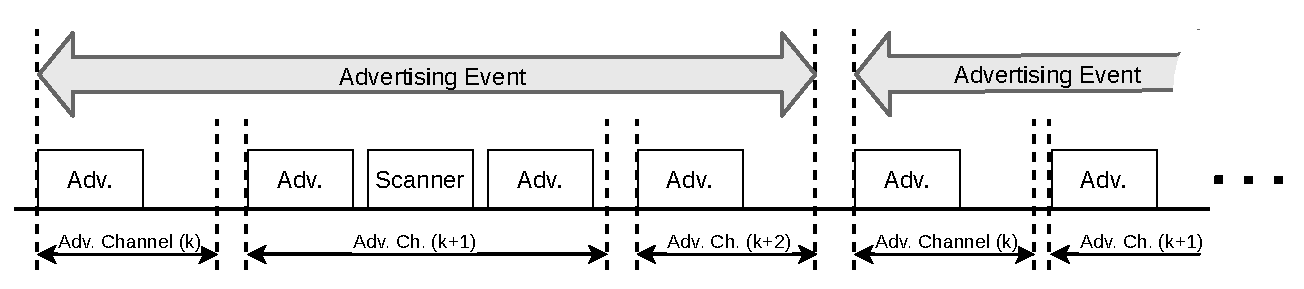
\includegraphics[width=\textwidth]{graphics/advertising_event.pdf}
    \caption[Advertising Event]{Advertising Event \cite{BtSpec4.0_127}}
    \label{fig: adv event}
\end{figure}
% QUELLE Spec S. 127 oben

In Abb. \ref{fig: adv event} ist ein Advertising Event dargestellt, bei dem ein Advertiser auf allen drei Advertising Channels nacheinander Advertisement-Pakete sendet. Auf dem zweiten Kanal empfängt der Advertiser -direkt im Anschluss auf sein erstes Advertisement-Paket- in diesem Kanal ein Paket eines Scanners, auf das er mit einem weiteren Advertisement antwortet.

\begin{figure}[H]
    \centering
    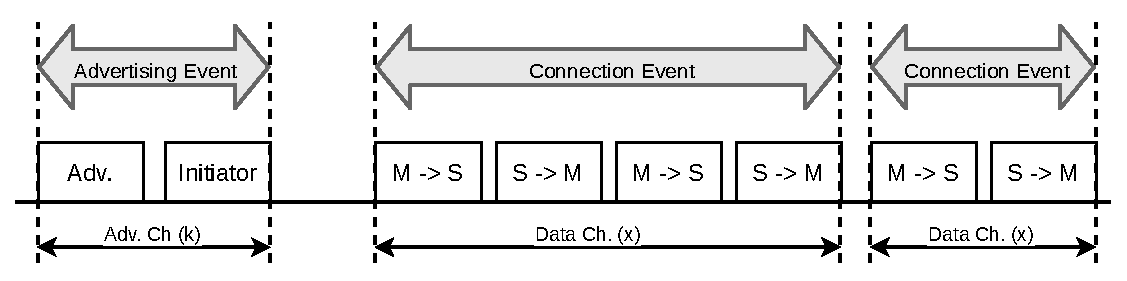
\includegraphics[width=0.9\textwidth]{graphics/advertising_initiator_event.pdf}
    \caption[Advertising und Connection Event]{Advertising und Connection Event \cite{BtSpec4.0_127}}
    \label{fig: adv init}
\end{figure}
% QUELLE Spec S. 127 unteres bild

In Abbildung \ref{fig: adv init} ist ein Advertising Event dargestellt, bei dem ein Initiator auf das Advertisement-Paket eines Advertiser antwortet, um eine Verbindung aufzubauen. Darauf folgt ein Connection Event, bei dem Master (ursprünglich Initiator) und Slave (ursprünglich Advertiser) einander Pakete auf einem Data Channel senden. Danach folgt ein weiteres Connection Event auf einem anderen Data Channel.

\newpage
\section{Implementierung}
	\label{sec: impl allg}
	Mithilfe der definierten Infrastruktur kann nun eine Implementierung für einen spezifischen Anwendungsfall erstellt werden. In dieser Arbeit wird die Infrastruktur auf einen autonomen Verleih von elektrischen Kleinfahrzeugen in Bezug auf das Projekt \textit{SteigtUM} (siehe Sektion \ref{sec: einleitung}) angewandt. Der Verleihdienst sieht vor, dass ein Benutzer mit einem Smartphone ein Kleinfahrzeug ausleihen kann. Smartphone und Kleinfahrzeug (Mikrocontroller) kommunizieren mittels BLE miteinander. Um einen Ausleihprozess einzuleiten wird ein Back End in Form eines Servers benötigt, damit ein Verwaltungsmodell realisiert werden kann. Dieses Modell ist jedoch nicht Bestandteil der Arbeit. Dennoch wird für den Prototyp (und für die spätere reale Implementierung) ein Back End benötigt, um den Benutzer bzw. die Smartphone-Anwendung (App) zum Ausleihen eines Fahrzeugs zu autorisieren.
\\\\
Innerhalb des Prototyps kommunizieren anstelle eines Smartphones und eines Mikrocontrollers vorerst nur zwei Mikrocontroller. Ein Mikrocontroller wird mit dem Verleihfahrzeug assoziiert, während der andere das Smartphone des Benutzers vertritt. Die weiteren Kommunikationsparteien Back End und Zertifizierungsstelle werden simuliert.
\\\\
Für die Implementierung wurden einige Bedingungen aufgestellt, damit sie das konkrete Modell eines Verleihdienstes nicht einschränkt. Eine Bedingung ist, dass zu Beginn eines Ausleihprozesses die App mit dem Back End kommunizieren kann, bis der Benutzer das Fahrzeug nutzen kann. Danach darf keine weiter bestehende Verbindung zwischen App und Back End vorausgesetzt werden. Zwischen dem Fahrzeug und dem Back End darf nie eine Verbindung vorausgesetzt werden. Wird die Bluetooth-Verbindung zwischen App und Fahrzeug unterbrochen, darf nicht davon ausgegangen werden, dass zwischen App und Back End eine (sichere) Verbindung hergestellt werden kann. Somit bleibt die Implementierung weitestgehend unabhängig von äußeren Einflüssen, die die Verbindungen zum Back End beeinträchtigen können. Außerdem gibt sie nicht vor, welche technischen Voraussetzungen das Fahrzeug für die Kommunikation benötigt (mit Ausnahme von BLE).

	\subsection{Topologie}
		\label{sec: impl topologie}
		Die Topologie der Infrastruktur beschränkt sich auf das Minimum an Kommunikationsparteien und ist unabhängig von der Anwendung.\\

% TODO BILD topologie infratruktur mikrocontroller, smartphone, CA

Dem Thema zufolge sollen ein Mikrocontroller und ein Smartphone sicher Daten austauschen. Um dies zu bewerkstelligen, wird über den Transport der Daten durch Bluetooth Low Energy (BLE) das Verschlüsselungsprotokoll TLS verwendet (siehe Sektion X). 
% TODO SEKTION VERWEIS Infrakstruktur->Sicherheit
Dementsprechend ist, wie in Abbildung X zu sehen
% TODO BILD VERWEIS topologie infrastruktur mikrocontroller, smartphone, CA
, neben dem Mikrocontroller und dem Smartphone eine Zertifizierungsstelle notwendig. In welcher Form diese auftritt ist von der Anwendung abhängig.

Für einen seriösen Anwendungsfall sollte die Zertifizierungsstelle evtl. in Form eines Servers existieren, der dem Mikrocontroller und Smartphone in regelmäßigen Abständen (z.B. jährlich) jeweils ein Zertifikat ausstellt. Mit diesen Zertifikaten und der Kenntnis über das Root-Zertifikat können Mikrocontroller und Smartphone sich gegenseitig authentifizieren und somit die Grundlage für eine sichere Kommunikation bilden.

Beispielsweise könnte es für einen privaten Anwendungsfall ausreichend sein, die Zertifizierungsstelle nicht als dauerhaft betriebenen Server darzustellen, sondern lediglich ein Root-Zertifikat zu erstellen und mit diesem dem Mikrocontroller und Smartphone jeweils ein digitales Zertifikat auszustellen.

Die Rolle der Partei, die die Zertifikate für Mikrocontroller und Smartphone austellt muss nicht zwingend eine Zertifizierungsstelle sein, sondern könnte auch eine Entität sein, der von einer Zertifizierungsstelle ein Zwischenzertifikat ausgestellt wurde.

	\subsection{Ausleihprozess}
		\label{sec: impl ausleih allg}
		Mit der Anwendung der Infrastruktur wird bereits der Aufbau einer sicheren Verbindung zwischen Smartphone und Mikrocontroller ermöglicht. Ab diesen Punkt muss der Mikrocontroller sicherstellen, dass der Benutzer bzw. das Smartphone dazu autorisiert ist, das Fahrzeug auszuleihen. Dieses Problem wird mit einer vom Back End signierten Bestätigung gelöst, die im Rahmen dieser Arbeit als "`Subscription"' bezeichnet wird.
\\\\
Die Subscription muss folgende Anforderungen erfüllen. Sie muss beweisen, dass sie ausschließlich vom Back End angefertigt wurde (Authentizität). Falls ihr Inhalt von einer anderen Instanz verändert wurde, muss dies bei der Prüfung der Subscription ersichtlich werden (Datenintegrität). Die Informationen innerhalb der Subscription beziehen sich auf den zugehörigen Ausleihvorgang (z.B. Identität des Fahrzeugs/Mikrocontrollers, Zeitstempel).

		\subsubsection{Verbindungsaufbau und Autorisierung}
			\label{sec: impl verbindungsaufbau und autorisierung}
			Bevor die Subscription erstellt bzw. vom Smartphone angefordert wird, herrscht folgende Ausgangssituation. Vor der Inbetriebnahme des Verleihdienstes müssen Smartphone, Back End und Mikrocontroller jeweils über ein individuelles Zertifikat (nach X.509-Standard) und dessen privaten Schlüssel verfügen. Die Zertifikate wurden jeweils von der Zertifizierungsstelle ausgestellt. Zudem kennt auch jede der drei Parteien (Smartphone, Back End, Mikrocontroller) das Root-Zertifikat (das Zertifikat der Zertifizierungsstelle), um damit die anderen Parteien authentifizieren zu können. Außerdem benötigt das Back End ein weiteres Zertifikat mit zugehörigem privaten Schlüssel, das Subscription-Zertifikat genannt wird.
\\\\
Nun möchte ein Nutzer mit der Smartphone-Anwendung (App) ein Fahrzeug ausleihen. Dafür sollte das Fahrzeug signalisieren, dass es für einen Ausleihvorgang zur Verfügung steht. Ab diesen Punkt ist der weitere Verlauf des Ausleihprozesses in Abb. \ref{fig: verlauf ausleihprozess} dargestellt.
\begin{figure}[H]
    \centering
    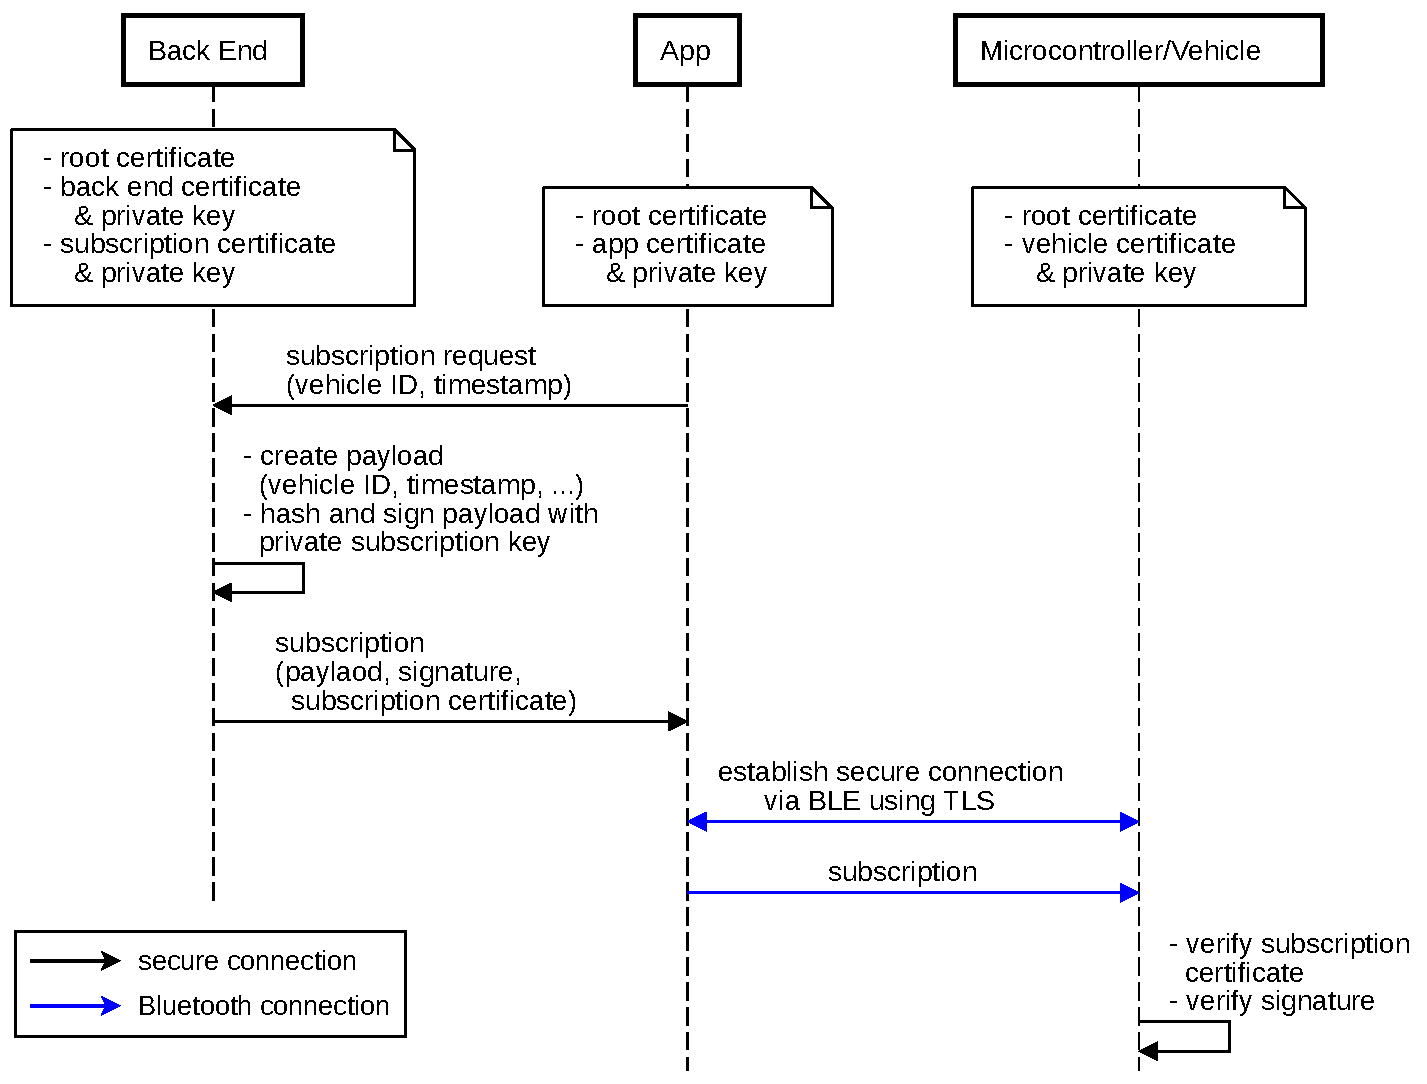
\includegraphics[width=1\textwidth]{graphics/verlauf_ausleihprozess.pdf}
    \caption[Verlauf des Ausleihprozzeses]{Verlauf des Ausleihprozzeses}
    \label{fig: verlauf ausleihprozess}
\end{figure}
Zu Beginn muss die App die Identität und Bluetooth-Adresse des Fahrzeugs feststellen (z.B. über einen Quick Response Code, kurz QR-Code). Die App baut eine sichere Verbindung zum Back End auf und verlangt nach einer Subscription. Dabei sendet sie die Identität des Fahrzeugs, einen aktuellen Zeitstempel und evtl. weitere Informationen (z.B. bzgl. des Bezahlmodells). Das Back End fügt zu diesen Informationen evtl. noch weitere hinzu (z.B. bzgl. des Bezahlmodells) und formt daraus den "`Payload"'. Danach wird der Hashwert des Payloads gebildet und mit dem privaten Schlüssel signiert. Die Subscription setzt sich nun entsprechend Abb. \ref{fig: aufbau subscription} zusammen.
\begin{figure}[H]
    \centering
    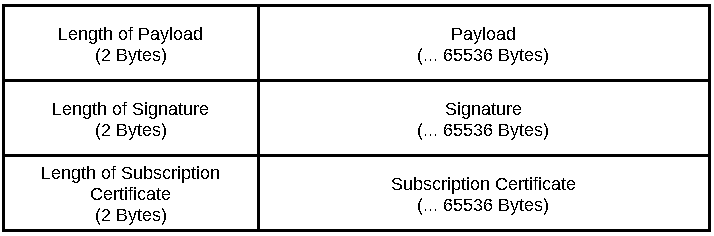
\includegraphics[width=0.9\textwidth]{graphics/aufbau_subscription.pdf}
    \caption[Aufbau der Subscription]{Aufbau der Subscription}
    \label{fig: aufbau subscription}
\end{figure}
Das erste Längenfeld gibt die Länge des darauffolgenden Payloads an. Das zweite Längenfeld gibt die Länge der Signatur an, worauf die Signatur folgt. Das letzte Längenfeld steht für die Länge des Subscription-Zertifikats und ist gefolgt vom Subscription-Zertifikat. Schließlich überträgt das Back End die Subscription an die App und trennt die Verbindung.
\\\\
Entsprechend der Sektion \ref{sec: infra verbindungsaufbau} verbindet sich die App über BLE mit dem Fahrzeug und stellt mittels TLS eine sichere Verbindung her. Daraufhin beendet das Fahrzeug das Advertising. Anschließend sendet die App die Subscription an das Fahrzeug. Zuerst verifziert das Fahrzeug das Subscription-Zertifikat, indem es dessen Signatur mit dem Root-Zertifikat prüft. Danach verifiziert es die Signatur des Payloads mit der gleichen Hash-Funktion, die zur Erstellung der Signatur genutzt wurde, und dem öffentlichen Schlüssel des Subscription-Zertifikats. Sind die Verifikationen erfolgreich, konnte das Fahrzeug sicherstellen, dass die Subscription vom Back End erstellt wurde. Nun müssen noch die Inhalte des Payloads geprüft werden. Demnach muss die angegebene Identität mit der des Fahrzeugs übereinstimmen und der Zeitstempel aktuell sein. Wurden weitere Informationen angegeben, sollte deren Plausibilität geprüft deren Informationsgehalt verarbeitet werden. Somit ist der erste Teil des Ausleihprozesses abgeschlossen. Sollte eine der Verifikationen fehlschlagen sowohl bei der Prüfung der Subscription als auch vorher auf Ebene von TLS, wird die Verbindung abgebrochen.

		\subsubsection{Erneuter Verbindungsaufbau}
			\label{sec: impl erneuter verbindungsaufbau}
			Ab diesen Punkt muss ein weiterer Fall für den Verlauf des Ausleihprozesses berücksichtigt werden: der Abbruch der Verbindung zwischen Smartphone und Fahrzeug sowie die darauffolgende Wiederherstellung der Verbindung. Der Verbindungsabbruch kann zum einen durch technische Einflüsse (z.B. Interferenzen) verursacht werden und nicht vom Benutzer beabsichtigt sein. Zum anderen ist es denkbar, dass der Nutzer sich für eine bestimmte Zeitspanne vom Fahrzeug entfernt, wodurch die Verbindung aufgrund der begrenzten Bluetooth-Reichweite abbricht. Evtl. sollte hier der Benutzer dem Fahrzeug signalisieren, dass er für eine bestimmte Zeitspanne abwesend ist. Danach begibt sich der Nutzer wieder zum Fahzeug und möchte es weiter nutzen.
\\\\
Wenn die Verbindung nun abbricht, beginnt das Fahrzeug mit dem Advertising. Sobald der Benutzer bzw. das Smartphone in Reichweite ist, verbindet sich die App per BLE mit dem Fahrzeug, da es die Bluetooth-Adresse des Fahrzeugs bereits kennt, und baut wie oben beschrieben eine sichere Verbindung auf. Nun sendet die App die alte Subscription erneut an das Fahrzeug. Das Fahrzeug prüft erneut die Subscription und vergleicht sie mit der Subscription, die es zu Beginn des Ausleihprozesses empfangen hat. Wurde die Subscription erfolgreich verifiziert und stimmt sie mit der ursprünglichen Subscription überein, kann das Fahrzeug wieder genutzt werden.

		\subsubsection{Beenden des Ausleihprozesses}
			\label{sec: impl beenden des ausleihprozesses}
			Das Beenden des Ausleihprozesses ist mitunter abhängig vom Bezahlmodell des Verleihdienstes. Im Wesentlichen könnte die App dem Fahrzeug eine Nachricht senden, die besagt, dass der Ausleihprozess nun beendet wird. Zudem sollte auch der Fall berücksichtigt werden, wenn keine ordnungsgemäße Beendigung stattfindet. Dabei sollte sich das Fahrzeug nach einer bestimmten Zeitspanne für neue Ausleihprozesse automatisch freigegeben.

		\subsubsection{Einfluss der Infrastruktur}
			\label{sec: impl einfluss der infrastruktur}
			Da die Zertifikate der Parteien (Back End, App, Fahrzeug) von der Zertifizierungsstelle des Verleihdienstes ausgestellt wurden und die Parteien nur das Root-Zertifikat des Verleihdienstes nutzen, um das Zertifikat eines Gegenüber zu verifizieren, können nur die Parteien TLS-Verbindungen zueinander aufbauen. Jede außenstehende Instanz, die versucht eine Verbindung zu einer der Parteien (Back End, App, Fahrzeug) aufzubauen, wird bereits beim TLS-Handshake abgewiesen. Grund dafür ist, dass die außenstehende Instanz kein von der Zertifizierungsstelle ausgestelltes Zertifikat besitzt. Sollte sie doch an ein solches Zertifikat gelangen, muss sie beim TLS-Handshake immer noch beweisen, dass sie den zugehörigen privaten Schlüssel besitzt. Aus diesem Grund muss jede der Parteien (Back End, App, Fahrzeug) den privaten Schlüssel geheim halten. Das bedeutet auch, dass ein Angreifer nicht in der Lage sein darf, den privaten Schlüssel aus einer der Parteien auszulesen (z.B. bei physischen Zugang). Deshalb sollten Zertifikate und private Schlüssel in Keystores gespeichert werden.

	\subsection{Prototyp}
		\label{sec: impl prototyp allgemein}
		In diesem Abschnitt werden Details zum Prototyp angegeben. Wie bereits erwähnt, ist der Prototyp nicht für eine Smartphone-Anwendung und einen Mikrocontroller umgesetzt, sondern vorerst nur für zwei Mikrocontroller. Dabei vertritt ein Mikrocontroller die Rolle der Smartphone-Anwendung (Client-Mikrocontroller) und der andere die Rolle des Fahrzeugs (Server-Mikrocontroller)).
\\\\
Im Anhang \ref{sec: anhang} ist das zugehörige Repository verlinkt.

		\subsubsection{Hardware und Software}
			\label{sec: impl soft hard}
			Zur Entwicklung des Prototyps wurde neben einem Personal Computer (PC) folgende Hardware verwendet:

\begin{itemize}
    \item Mikrocontroller \textit{ESP32-WROOM-32}
    \item Smartphone mit Android 11.0
\end{itemize}

Obwohl das Smartphone vorerst nicht Teil des Prototyps ist, wird es bzw. das Betriebssystem \textit{Android} einbezogen.

\subsubsection{ESP32-WROOM-32 (Mikrocontroller)}
Der \textit{ESP32-WROOM-32} unterstützt Bluetooth 4.2 für BR/EDR und BLE \cite{ESP32_6}. Der Hersteller \textit{Espressif} stellt das \textit{Espressif Internet of Things Development Framework} (ESP-IDF) \cite{ESPIDF}, mit dem Anwendungen für den \textit{ESP32-WROOM-32} entwickelt werden können. Das ESP-IDF unterstützt unter anderem folgende Software-Komponenten:

\begin{itemize}
    \item \textit{Free Real Time Operating System} (FreeRTOS)
    \item \textit{Serial Peripheral Interface Flash Files System} (SPIFFS)
    \item \textit{nimBLE}
    \item \textit{mbedTLS}
\end{itemize}

FreeRTOS dient als Betriebssystem für den \textit{ESP32-WROOM-32}. SPIFFS wird benötigt, um Dateien auf den \textit{ESP32-WROOM-32} zu "`flashen"' bzw. um auf diese während der Laufzeit zugreifen zu können.

\textit{nimBLE} ist eine Software-Bibliothek für den BLE-Host von der \textit{Apache Software Foundation} und bietet Programmierschnittstellen für GAP und L2CAP \cite{nimBLE}. Für GAP und L2CAP wird jeweils ein Event Handling ausgeführt. So kann bspw. festgelegt werden, welche Reaktion auf das Entdecken eines anderen Bluetooth-Geräts folgt oder wie mit über L2CAP empfangenen Anwendungsdaten verfahren wird.

\textit{mbedTLS} ist eine Software-Bibliothek für TLS und eignet sich aufgrund niedriger Anforderungen an den Speicher für eingebettete Systeme. Aktuell wird höchstens TLS 1.2 unterstützt \cite{ArmMbedCoreFeatures}.

\subsubsection{Smartphone/Android}
Das Smartphone unterstützt Bluetooth 5.0 und wird mit Android 11.0 betrieben. Wenn es mit dem \textit{ESP32-WROOM-32} per Bluetooth kommuniziert, wird also die Bluetooth-Version 4.2 verwendet. Android unterstützt mit den Programmpaketen "`android.bluetooth.le"' \cite{android_le} BLE und mit "`javax.net.ssl"' \cite{android_ssl} SSL/TLS. Wie in Sektion \ref{sec: infra sicherheit} erläutert, sollten nur TLS 1.2 oder TLS 1.3 genutzt werden. TLS 1.2 wird ab Android 4.1 und TLS 1.3 ab Android 10.0 unterstützt \cite{android_ssl_context}.

		\subsubsection{Simulierung der Zertifizierungsstelle}
			\label{sec: impl prototyp zertifizierungstelle}
			Die Zertifizierungstelle wird mittels eines Personal Computer (PC) simuliert. Die Zertifikate und Schlüssel werden vom PC mittels \textit{mbedTLS} generiert und beim "`Flashen"' des jeweiligen Programmes auf die Mikrocontroller als Dateien übertragen. Jedoch werden sie nicht in Keystores gespeichert. Die Zertifkate werden nach dem Standard X.509 erstellt und die Schlüssel mittels des RSA-Verfahrens generiert. In Abb. \ref{fig: impl certs keys} wird gezeigt, wie sie erstellt bzw. generiert werden.
\begin{figure}[H]
    \centering
    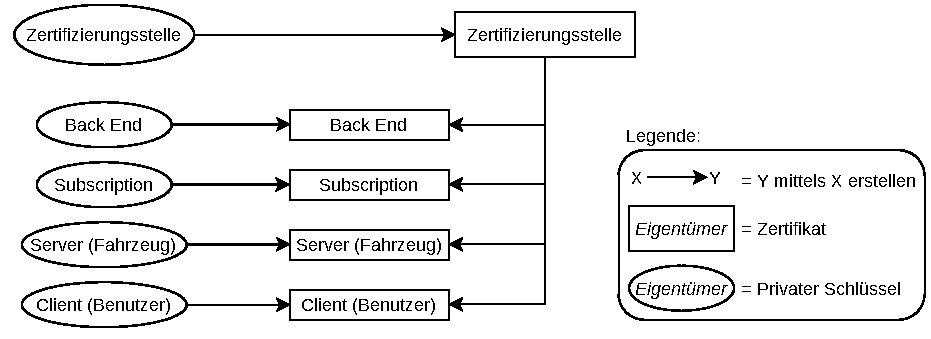
\includegraphics[width=0.9\textwidth]{graphics/impl_keys_certs.pdf}
    \caption[Generierung der Schlüssel und Erstellung der Zertifikate]{Generierung der Schlüssel und Erstellung der Zertifikate}
    \label{fig: impl certs keys}
\end{figure}
Zuerst wird ein 4096 Bit langer privater Schlüssel für die Zertifizierungsstelle generiert. Danach wird das zugehörige Root-Zertifikat mit diesem Schlüssel erstellt. Dabei wird angegeben, dass es ein selbstunterzeichnetes Zertifikat ist und für eine Zertifizierungsstelle ausgestellt wird. Der Name des Ausstellers ist in diesem Fall auch der Name des Eigentümers. Alle weiteren privaten Schlüssel sind ebenfalls 4096 Bit lang. Wurden sie generiert, wird mit jedem privaten Schlüssel genau ein Zertifikat erstellt, dessen Ausstellerzertifikat das Root-Zertifikat ist.
\\\\
Nun liegen alle Zertifikate und Schlüssel vor und werden beim "`Flashen"' des jeweiligen Programmes folgendermaßen auf die beiden Mikrocontroller übertragen:
\begin{itemize}
    \item Server-Mikrocontroller (Fahrzeug):
    \begin{itemize}
        \item privater Server-Schlüssel (Fahrzeug)
        \item Server-Zertifikat (Fahrzeug)
        \item Root-Zertifikat
    \end{itemize}
    \item Client-Mikrocontroller (stellvertretend für die App):
    \begin{itemize}
        \item privater Client-Schlüssel (App)
        \item Client-Zertifikat (App)
        \item privater Subscription-Schlüssel
        \item Subscription-Zertifikat
        \item Root-Zertifikat
    \end{itemize}
\end{itemize}
Der Client erhält zusätzlich den Schlüssel und das Zertifikat zum Erstellen der Subscriptions, um so das Back End zu simulieren.

		\subsubsection{Ablauf der Anwendung für Client und Server}
			\label{sec: impl prototyp anwendung}
			Entsprechend Abb. \ref{fig: impl ablauf anwendung teil 1} ist der erste Teil des Ablaufs der Anwendungen für Client-Mikrocontroller bzw. Server-Mikrocontroller dargestellt. Er ist für beide Anwendungen identisch.
\begin{figure}[H]
    \centering
    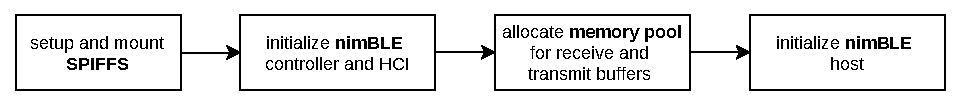
\includegraphics[width=1\textwidth]{graphics/ablauf_anwendung_teil_1.pdf}
    \caption[Ablauf beider Anwendungen (Teil 1)]{Ablauf beider Anwendungen (Teil 1)}
    \label{fig: impl ablauf anwendung teil 1}
\end{figure}
Zu Beginn wird das Dateisystem SPIFFS konfiguriert und initialisiert. Vor dem "`Flashen"' wird eine Partition erstellt, die die jeweiligen Schlüssel und Zertifikate enthält (siehe Sektion \ref{sec: impl prototyp zertifizierungstelle}). Danach wird über \textit{nimBLE} der Bluetooth-Controller im Modus Low Energy und das Host Controller Interface initialisert. Danach wird Speicher für zwei Memory Pools reserviert: einen Memory Pool für empfangene Anwendungsdaten und einen für zu sendende Anwendungsdaten. Schließlich wird der nimBLE-Host in einem neuen Task initialisiert, um das Event Handling für L2CAP und GAP separiert von der Anwendung zu betreiben.
\\\\
Die Abb. \ref{fig: impl ablauf anwendung server teil 2} zeigt den weiteren Ablauf der Server-Anwendung.
\begin{figure}[H]
    \centering
    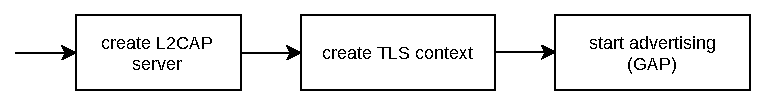
\includegraphics[width=0.8\textwidth]{graphics/ablauf_anwendung_teil_2_server.pdf}
    \caption[Ablauf der Server-Anwendung (Teil 2)]{Ablauf der Server-Anwendung (Teil 2)}
    \label{fig: impl ablauf anwendung server teil 2}
\end{figure}
Zunächst wird der L2CAP-Server erstellt und somit wird das L2CAP Event Handling aktiv. Danach wird der TLS-Kontext erstellt. Er benötigt den privaten Schlüssel und das Zertifikat des Fahrzeugs sowie das Root-Zertifikat. Zudem verlangt er nach den Funktionen für das Senden bzw. Empfangen von Daten durch den Transport (L2CAP). Danach beginnt die Server-Anwendung mit dem Advertising mithilfe von GAP. Dabei werden Connectable Undirected Advertising Events als Broadcast gesendet, in denen die öffentliche Bluetooth-Adresse des Server-Mikrocontrollers angegeben wird. Nun ist auch das GAP Event Handling aktiv.
\\\\
In Abb. \ref{fig: impl ablauf anwendung client teil 2} ist der weitere Ablauf der Client-Anwendung dargestellt.
\begin{figure}[H]
    \centering
    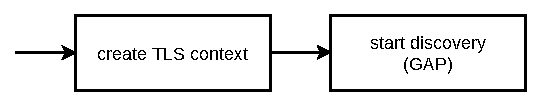
\includegraphics[width=0.6\textwidth]{graphics/ablauf_anwendung_teil_2_client.pdf}
    \caption[Ablauf der Client-Anwendung (Teil 2)]{Ablauf der Client-Anwendung (Teil 2)}
    \label{fig: impl ablauf anwendung client teil 2}
\end{figure}
Die Client-Anwendung erstellt ebenfalls einen TLS-Kontext, nur dass hier der private Schlüssel und das Zertifikat für den Client und nicht für das Fahrzeug benötigt wird. Danach wird mittels GAP nach Advertising Events gescannt (General Discovery Mode) und somit wird das GAP Event Handling aktiv.
\\\\

% BLE verbinung
% TLS
% verweis auf emulation des back ends für subscription austausch
% RX buffer management

		\subsubsection{Simulierung des Back Ends}
			\label{sec: impl prototyp back end}
			\input{sections/implementierung/prototyp/simulierung_des_backends.tex}

\newpage
\section{Ausblick}
	% TODO

\newpage
\section{Zusammenfassung}
	Zu Beginn der Arbeit wurde die Funktionsweise von \textit{Bluetooth Low Energy} (BLE) vorgestellt. Die Recherche beschränkte sich auf die Spezifikationen und Webauftritte der Bluetooth SIG, um aus erster Hand ein Verständnis für die BLE-Architektur zu gewinnen. Durch die Untersuchung der Sicherheitsfunktionen und weitere Recherche, konnten die Schwachstellen von BLE aufgedeckt werden.
\\\\
Zum Entwurf der Infrastruktur musste zunächst ein geeigneter Transport innerhalb der BLE-Architektur bestimmt werden. Die Tatsache, dass sich viele Quellen zu dieser Frage auf das Protokoll GATT beziehen, war irreführend. GATT ist aufgrund seiner Attributsemantik und dem einhergehenden Overhead in der Übertragung ungeeignet für den effizienten Transport von Daten. Stattdessen stellt sich L2CAP als geeignetes Transportprotokoll heraus. Desweiteren war eine Recherche bzgl. der Sicherheitprobleme der Kommunikation und deren Lösungen notwendig. Das TLS-Protokoll stellte sich dabei als hervorragende Lösung heraus, um über einen beliebigen Transport sicher Daten zu übertragen.
\\\\
Die Implementierung der Infrastruktur für den Verleihdienst wies das Problem der Autorisierung auf. Als Lösung wurde die "`Subscription"' entworfen, die sicherstellt, dass ein Nutzer berechtigt ist, ein Fahrzeug auszuleihen, und es nach kurzer Abwesenheit wieder zu nutzen. Der entwickelte Prototyp für die Implementierung zeigt, wie für zwei Mikrocontroller die Infrastruktur angewandt wird und eine Subscription sicher übertragen und verifiziert wird.
\\\\
Eine Weiterführung der Arbeit wäre in der Implementierung denkbar. Dabei könnte der Prototyp zunächst unter Einbezug eines Smartphones weiterentwickelt werden. Desweiteren könnten die Zertifizierungsstelle und der Back End Server physisch eingebunden werden, um einen realistischen Prototypen zu testen.

Außerdem kann die Arbeit mit einer genauen Kryptoanalyse des vorgestellten Konzepts der "`Subscription"' weitergeführt werden, um eventuelle Schwachstellen aufzudecken und auszuschließen.

\newpage
\printbibliography[heading=bibintoc]

\newpage
\appendix

\section{Beispiele}
	\subsection{Sequence Number / Next Expected Sequence Number}
		\label{sec: anhang nesn sn}
		\begin{figure}[H]
    \centering
    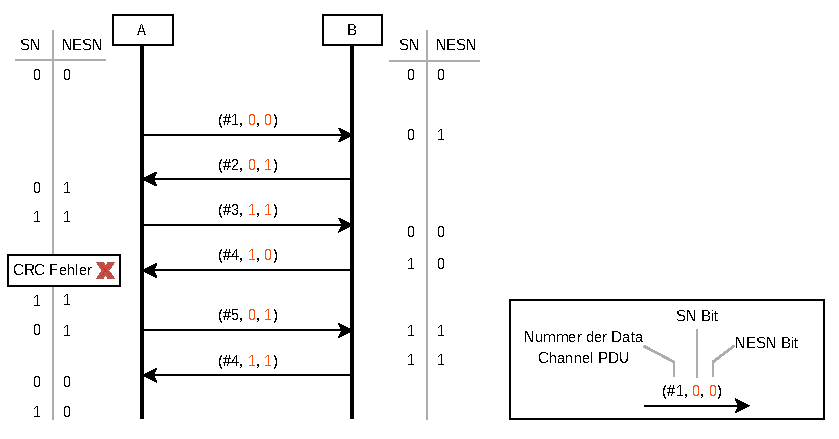
\includegraphics[width=0.9\textwidth]{graphics/nesn_sn_bsp.pdf}
    \caption[Beispiel für SN/NESN]{Beispiel für SN/NESN}
    \label{fig: anhang nesn sn}
\end{figure}

Gerät A und B verfügen jeweils über eigene Werte für SN/NESN und setzten diese jeweils auf 0 zu Beginn der Verbindung. Nun senden A und B gegenseitig Data Channel PDUs und nutzen folgenden Algorithmus für die SN/NESN. Die SN/NESN einer Data Channel PDU werden zur SN Bit bzw. NESN Bit genannt. Bei dem erstmaligen Empfang von Data Channel PDU \#4 gibt der CRC einen Fehler aus, also wurde das Paket nicht korrekt übertragen. 

Algorithmus zum Setzen der SN/NESN \cite{BtSpec4.0_2239-2241} (bezieht sich immer nur auf das ausführende Gerät):
\\\\
Sei "`neue Data Channel PDU"' eine Data Channel PDU, die erstmalig gesendet wird (also keine erneute Sendung einer bereits gesendeten Data Channel PDU).\\
Sei "`alte Data Channel PDU"' eine Data Channel PDU, die bereits von dem Gerät gesendet bzw. empfangen wurde.\\
Sei "`letzte Data Channel PDU"' eine Data Channel PDU, die das Gerät zuletzt gesendet hat.

\begin{itemize}
    \item Senden einer Data Channel PDU:
    \begin{enumerate}
        \item Setze NESN Bit auf NESN. Falls Data Channel PDU eine neue Data Channel PDU ist, setze SN Bit auf SN
    \end{enumerate}
    \item Empfangen einer Data Channel PDU:
    \begin{enumerate}
        \item Ist SN Bit gleich NESN, dann wurde eine neue Data Channel PDU empfangen und NESN wird inkrementiert. Anderenfalls ist SN Bit ungleich NESN, also wurde eine alte Data Channel PDU empfangen, die ignoriert wird.
        \item Ist NESN Bit ungleich SN, dann wurde die letzte Data Channel PDU vom gegenüber bestätigt (ACK) und es wird SN inkrementiert. Anderenfalls ist NESN Bit gleich SN, also wurde die letzte Data Channel PDU nicht bestätigt (NAK) und muss erneut gesendet werden. Dabei muss SN Bit den Wert des SN Bit der letzten Data Channel PDU (also die zuletzt vom Gerät gesendet wurde) annehmen.
    \end{enumerate}
\end{itemize}

% - senden neuer Daten: SN bit auf SN setzen
% - senden Daten: NESN bit auf NESN setzen

% - empfangen Daten:
% SN bit ==  NESN, dann wurden neue Daten empfangen, NESN ++
% SN bit != NESN, dann wurden alte Daten empfangen
% NESN bit != SN, dann zuletzt gesendete Daten wurden ack., SN++
% NESN bit == SN, dann zuletzt gesendete Daten nak, diese erneut senden
% und dabei SN bit auf den Wert der Data Channel PDU
% setzen, die nicht empfangen wurde

\section{Sequenzdiagramme}
	\subsection{Verbindungsaufbau der Infrastruktur}
		\label{sec: anhang infra verb aufbau}
		\begin{figure}[H]
    \centering
    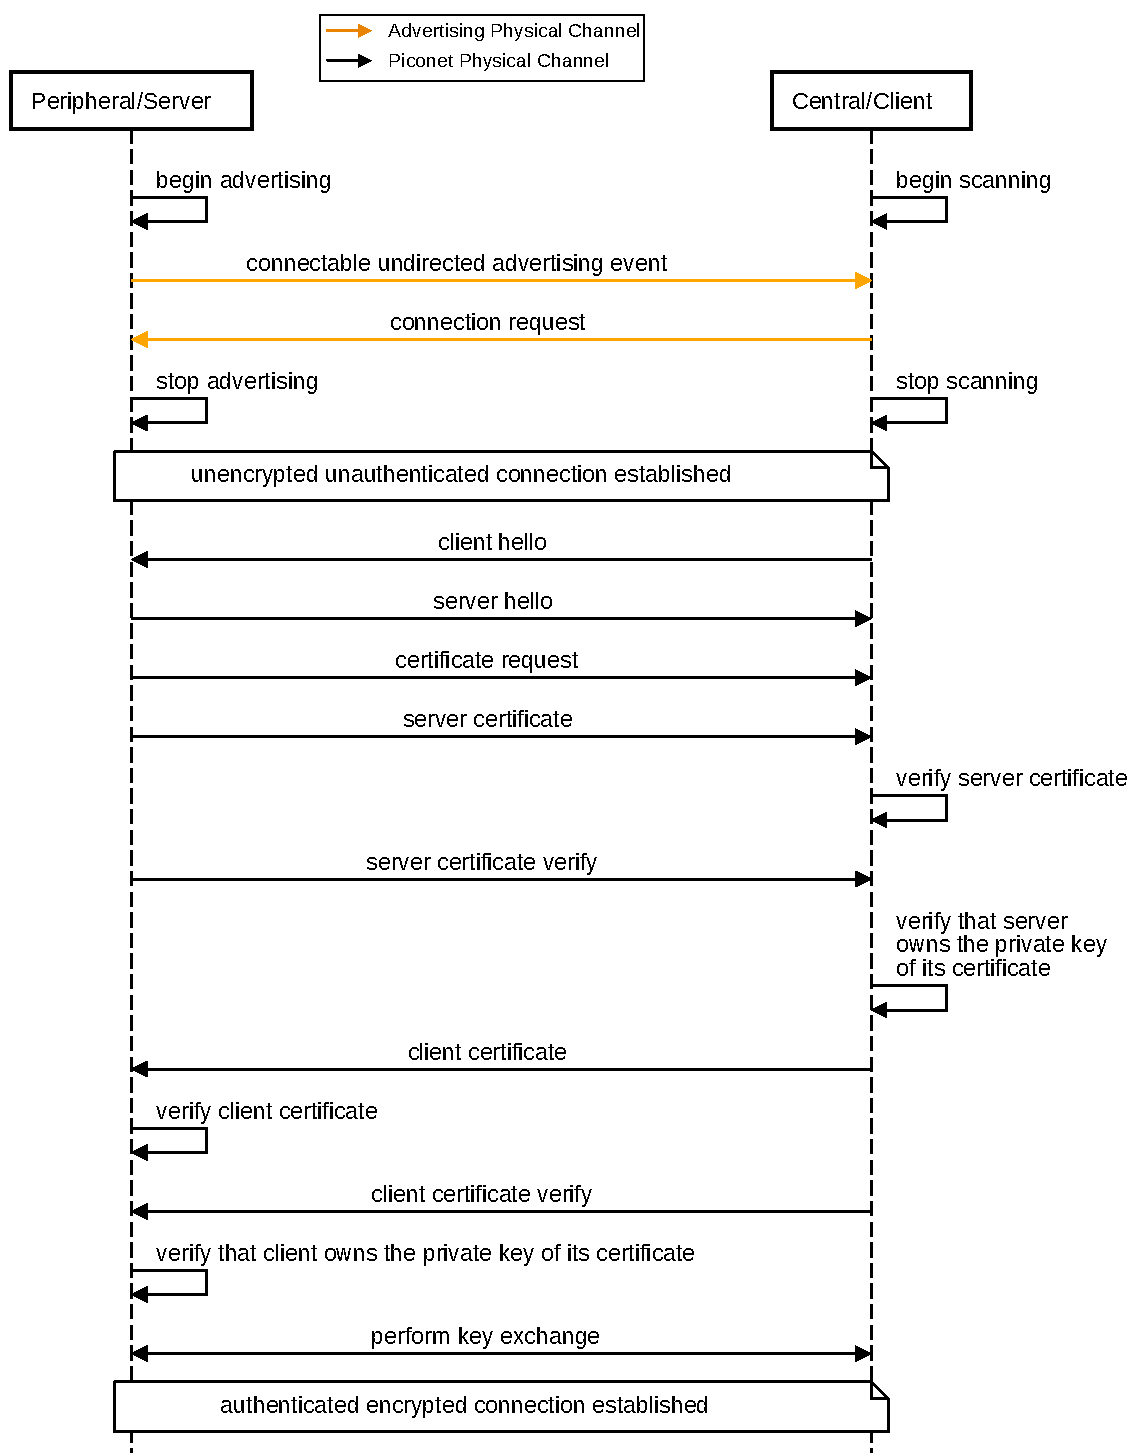
\includegraphics[width=1.05\textwidth]{graphics/infra_verb_aufbau.pdf}
    \caption[Verbindungsaufbau der Infrastruktur]{Verbindungsaufbau der Infrastruktur}
    \label{fig: infra verb aufbau}
\end{figure}

\end{document}